\documentclass[a4wide]{scrreprt}
\usepackage{a4wide}
\usepackage{ulem}
\usepackage{array}
\usepackage{graphicx}
\usepackage{hyperref}
\usepackage{float}

\newcommand{\comment}[1]{{\tt #1}}

\title{Kinect Controlled Robotic Arm}
\subtitle{System Requirements Specification}

\author{Aayush Singhal  (aayush@cse)    09005041 \and
        Sivakanth Gopi  (gopisivakanth@cse) 09005043 \and
        Sriram Bhargav Karnati  (ram@cse)   09005067 \and
        Aakash Rao N S  (aakash@cse)    09005069}
\date{}
\begin{document}
\maketitle

\tableofcontents
\chapter{Introduction}
The purpose of this document is to present a detailed description of the Kinect Controlled Robotic Arm. It will explain the purpose and features of the system, the interfaces of the system, what
the system will do, the constraints under which it must operate. This document is intended for the developers of the system.

\section{Definitions}



\begin{table}[h]
\setlength{\tabcolsep}{10pt}
%\centering
\noindent\makebox[\textwidth]{
\begin{tabular}{|m{0.16\textwidth}|m{0.75\textwidth}|}
\hline
\textbf{Term}& \textbf{Definition} \\
\hline
Robotic Arm & A programmable mechanical arm wih similar functions to a human arm\\
\hline
Arm & Unless specified otherwise, refers to the robotic arm \\
\hline
Kinect & A motion sensing input device developed by Microsoft\\
\hline
User & The person controlling the robotic arm\\
\hline
Depth Data & The data produced by the depth image camera in Kinect. Each frame in the stream contains the distance, in mm, to the nearest object at each x and y coordinate in the camera's field of view.\\
\hline
Skeletal Data & The data provided by Kinect about the configuration of a skeleton, as a set of positions that compose the sleleton. The skeleton represents the user's position and posture.\\
\hline
VGA & Video Graphics Accelerator \\
\hline
SDK & Software Development Kit \\
\hline
IDE & Integrated Development Environment \\
\hline
API & Application Programming Interface \\
\hline
GUI & Graphical User Interface \\
\hline 
DirectX & A collection of API for handling multimedia related tasks, on Microsoft platforms \\
\hline
AVR Studio & IDE for C programming for the robotic arm \\
\hline
IR & Infra-Red \\
\hline ZigBee & A specification for a suite of high level communication protocols using small, low-power digital radios based on an IEEE 802 standard for personal area networks \\
\hline 
X-CTU & Software used to configure the Zigbee wireless module \\
\hline
\end{tabular}}
\end{table}
\newpage

%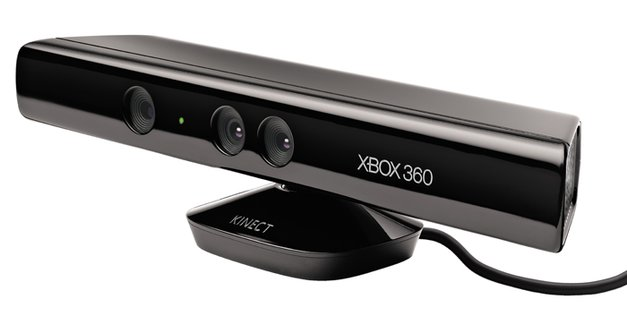
\includegraphics[scale=0.5]{kinect.jpg}
\begin{figure}[H]
\centering
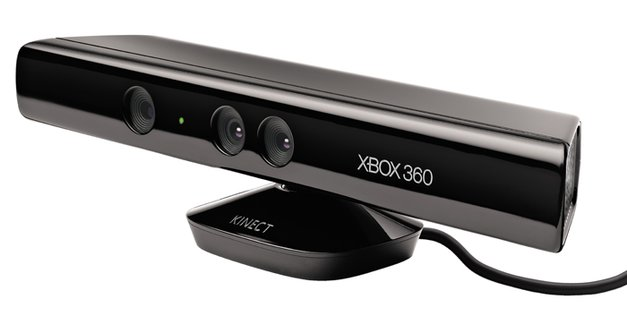
\includegraphics[scale=0.6]{kinect.jpg}
\caption{Microsoft Kinect} 
\end{figure}



\section{References}
\begin{itemize}
\item Kinect for Windows SDK v1 : Resources and Documentation, Microsoft Corporation\\ \url{http://www.microsoft.com/en-us/kinectforwindows/develop/resources.aspx}
\item Kinect SDK v1 Quick Starts, Channel 9, MSDN\\ \url{http://channel9.msdn.com/Series/KinectQuickstart} 
\item Dexter ER2 Robotic Arm User Manual, Nex Robotics, Version 1.00, April 2011\\ \url{http://www.nex-robotics.com/products/robotic-arms-and-grippers/dexter-er-2-heavy-duty-robotic-arm-with-controller-and-accessories.html}
\item AVR AtMega2560 Programming Manual, Atmel, May 2011 \\ \url{http://www.atmel.com/Images/doc2549.pdf}
\end{itemize}

%%%%%%%%%%%%%%%%%%%%%%%%%%%%%%%%%%%%%%%%%%%%%%%%%%%%%%%%%%%%%%%%%%%%%%%%%%%
\chapter{Overall Description}
%%%%%%%%%%%%%%%%%%%%%%%%%%%%%%%%%%%%%%%%%%%%%%%%%%%%%%%%%%%%%%%%%%%%%%%%%%%
\section{System Environment}
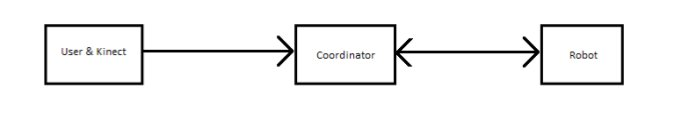
\includegraphics[scale=0.7]{pic0.jpg}\\
Kinect Controlled Robotic Arm has 2 active systems and 2 coordinating systems. Hand which is to be imitated, and robotic arm are active systems. And computer and kinect are coordinating systems. User's hand is able to communicate with robotic arm via coordinating systems. The communication between robotic arm and coordinating system is on a dedicated wireless frequency channel. While kinect is connected to computer by a wired connection.

\section{Product Perspective}
Kinect captures the movement and gestures of hand and body using its various sensors. Robotic arm is controlled remotely using ZigBee wireless interface. Computer receives hand movements from the kinect sensor and translates it to a particular command and sends that command to Robotic arm. Robotic arm looks as if, it is imitating the hand movement. 

In order to make the system completely remote control, a camera may be mounted on the top of robotic arm. So that user can view the environment of robotic arm from distance. Connection to Robotic arm can also be established without using ZigBee wireless device, and through a wired connection, because Robotic arm is kept stationary at all times.

\section{Product Functions}
\begin{figure}[htb]
\centering
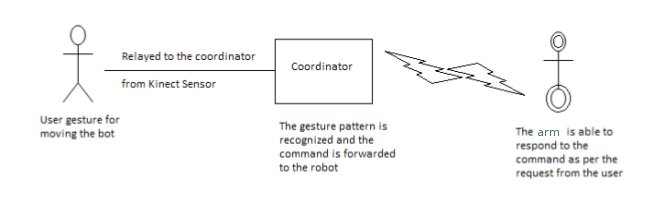
\includegraphics[scale=0.6]{pic2.jpg}
\caption{Robotic Arm Control Process}
\end{figure}
\subsection{Description}

The user moves hands to define some kind of commands to the robotic arm. 1 hand is to be imitated, while the other hand can be used to create gestures representing higher level instructions. The movements and gestures are described in Chapter 3. Whatever action of hand is captured by kinect, is translated into a instruction for robotic arm. Robotic arm doesn't have as many degrees of freedom as a hand, but it can reach any place a hand can reach because of its freedom in multiple directions. 

\subsection{Initial Step-By-Step Description}

To run it smoothly, the user must be recognized by kinect and wireless connection between robotic arm and computer must be active and strong enough to transmit commands and camera pictures through it.

\begin{enumerate}
\item The user performs movement of right hand in front of kinect sensor.
\item The user can make use of gestures by left hand to start/pause robotic arm from imitating actions of user's right hand.
\item The gestures and movements are recognized by kinect and computer and the command is forwarded to robotic arm on wireless.
\item Robotic arm accesses the command and performs the required task.
\item Robotic arm captures the environment around it using the camera and sends it via wireless to computer.
\item Pictures received from robotic arm are displayed on computer.
\end{enumerate}


\section{User Characteristics}

The user is expected to be able to perform the hand movements slowly taking good care that the kinect sensor is able to recognize the motion and ensure that most part of her arm is visible to the kinect sensor, so that it can be detected properly and analysed by the program on the coordinator which translated these motions into skeletal data. Main hand of user, which is to be imitated should not move around too fast, because kinect can capture around 10 frames per second, when arm is moving, and there is finite amount of lag between action and information. User should continuously monitor various interfacs presented to him, like the kinect sensor output, the skeletal data and the visual feed from the camera near the robotic arm.
\section{General Constraints}

\begin{enumerate}
\item The Kinect SDK is restricted to work on MS Windows 7 with DirectX SDK. Same will be the restrictions for the utility developed.
\item The Kinect Sensor Device requires a good processor and a dedicated VGA card. Same will be the requirements of the machine used as the coordinator.
\item The distance between the user and the kinect sensor must be 4 to 5 meters. The limit restriction is higher than that of kinect sensor, in order to prevent any interference from influencing the functioning of the Kinect Sensor. 
\item Hand should not be moved around too fast, depending on the bottleneck speed of utility, most probably decided by wireless connection or kinect processing speed.
\item Robotic arm cannot perform all kind of hand movements, as it doesn't have exactly same freedom degrees as hand, although it should be able to full-fill the ultimate purpose of reaching some space coordinate.
\end{enumerate}
\section{Potential Applications}
We intend to implement at least one of the following applications of the Kinect Controlled Robotic Arm (some of these may require implementation of additional features):
\begin{itemize}
\item Remote Bomb Diffusion Robot
\item Remotely controlled Crane with NUI
\item Writing/Painting using a Robotic Arm
\end{itemize}

 


\section{Requirement Subsets}

\begin{itemize}
\item Hand movement Detection
\item Hand gesture recognition
\item kinect and computer connection
\item Computer and ZigBee connection
\item ZigBee and Robotic arm connection
\item Interpretation and translation of commands
\item Mounting camera on suitable position on Robot
\item Map from hand movement to Robotic arm actions
\end{itemize}
%%%%%%%%%%%%%%%%%%%%%%%%%%%%%%%%%%%%%%%%%%%%%%%%%%%%%%%%%%%%%%%%%%%%%%%
\chapter{Robotic Arm Control}
%%%%%%%%%%%%%%%%%%%%%%%%%%%%%%%%%%%%%%%%%%%%%%%%%%%%%%%%%%%%%%%%%%%%%%%
The robotic arm is as shown in the figure. It has 6 axis of freedom corresponding to the 6 motors whose positions are shown. The movements corresponding to the 6 axis are presented in the table.
\begin{figure}[H]
\centering
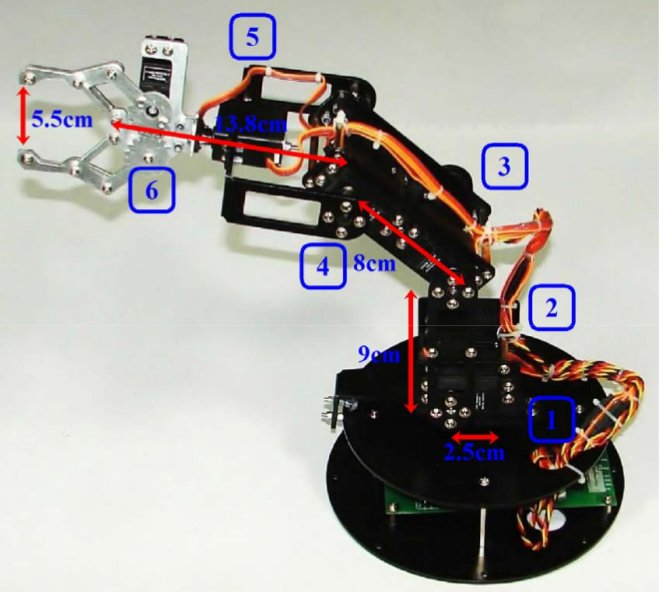
\includegraphics[scale=0.5]{arm-axes.jpg}
\end{figure}

\begin{figure}[H]
\centering
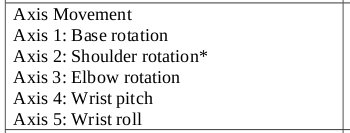
\includegraphics[scale=0.8]{arm-axes-table.jpg}
\end{figure}
We have to map these movements to the various gestures of the hands of the user. Below we describe the various gestures and their corresponding actions.
\section*{Start and Stop}
For this we can use the speech recognition capability of kinect. When the user says "start", the control of the robotic arm starts. When the user stays "stop", the control of the robotic arm ceases.
\section*{Zero Position}
This corresponds to the position of the robot relative to which all movements are done. We can change the zero position of the robot using the hold gesture.
\begin{figure}[H]
\centering
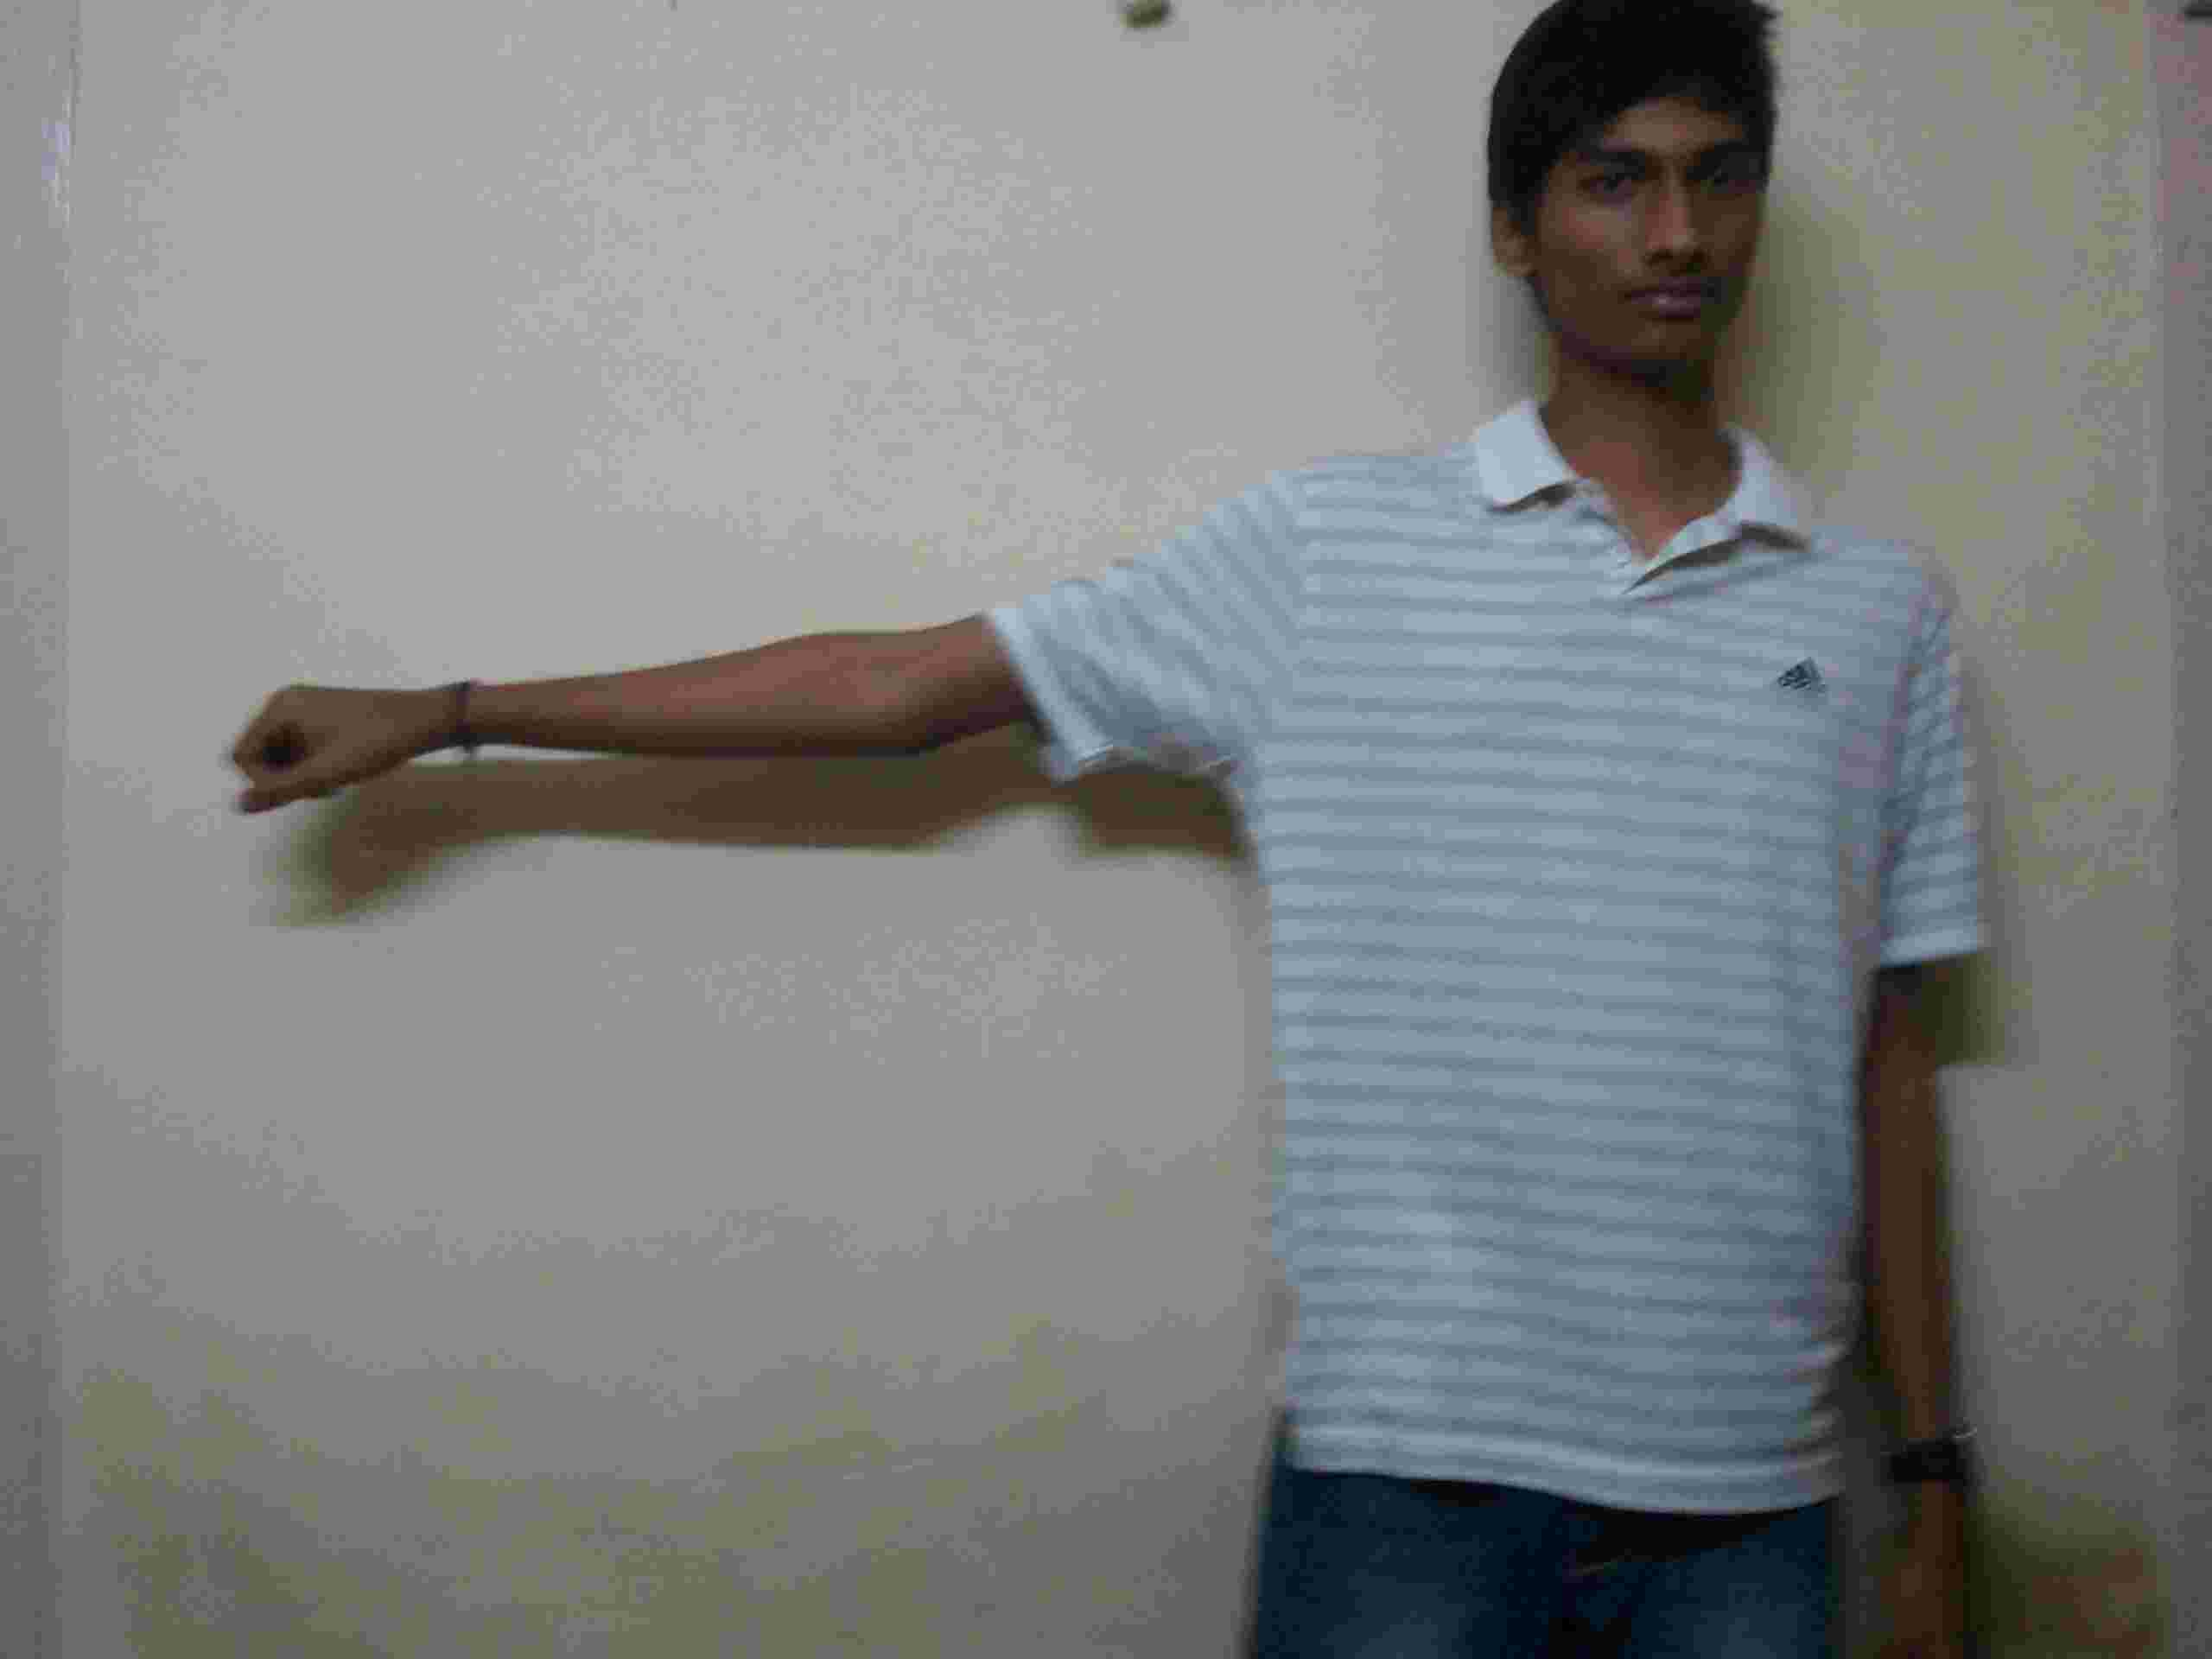
\includegraphics[scale=0.1]{gestures/0.jpg}
\end{figure}

\section*{Hold}
While we make the hold gesture, the control of the robotic arm stops temporarily. And this will make the current position of the robot to 'zero'. All further movements of the robotic arm will be relative to this 'zero' position.
\begin{figure}[H]
\centering
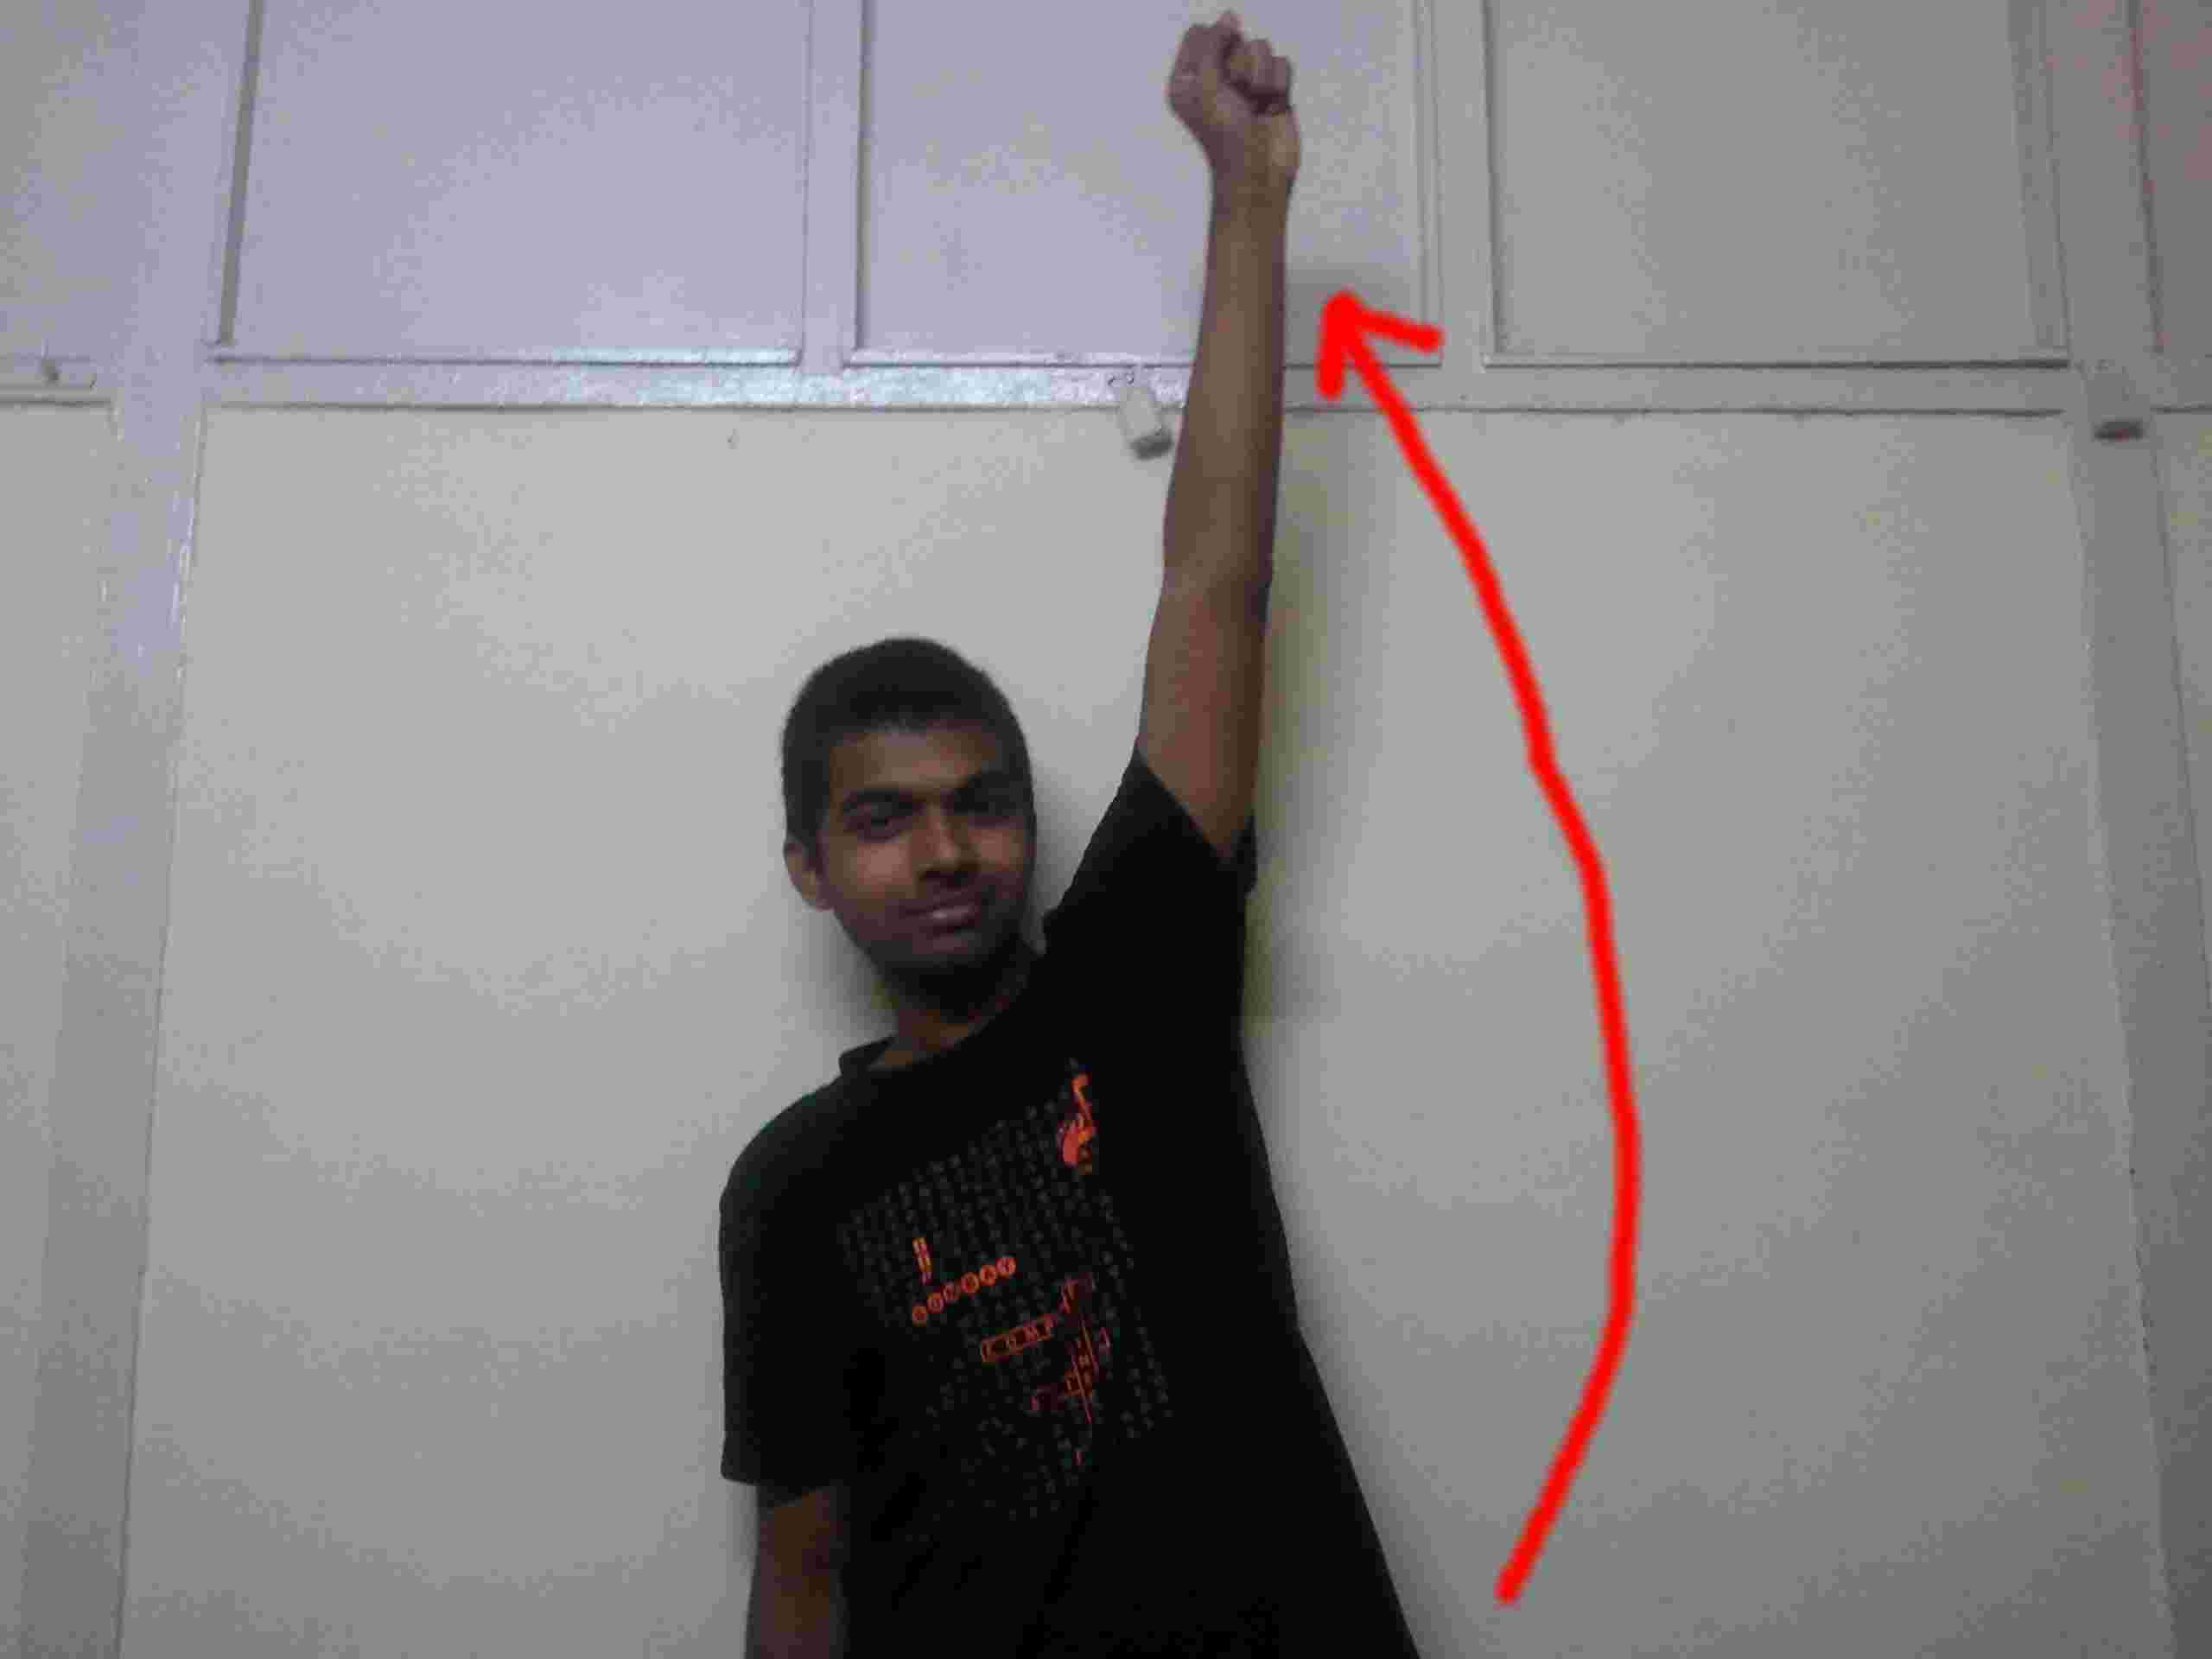
\includegraphics[scale=0.1]{gestures/hold.jpg}
\end{figure}
\section*{1.Base Rotation}
\begin{figure}[H]
\centering
$
\begin{array}{cc}
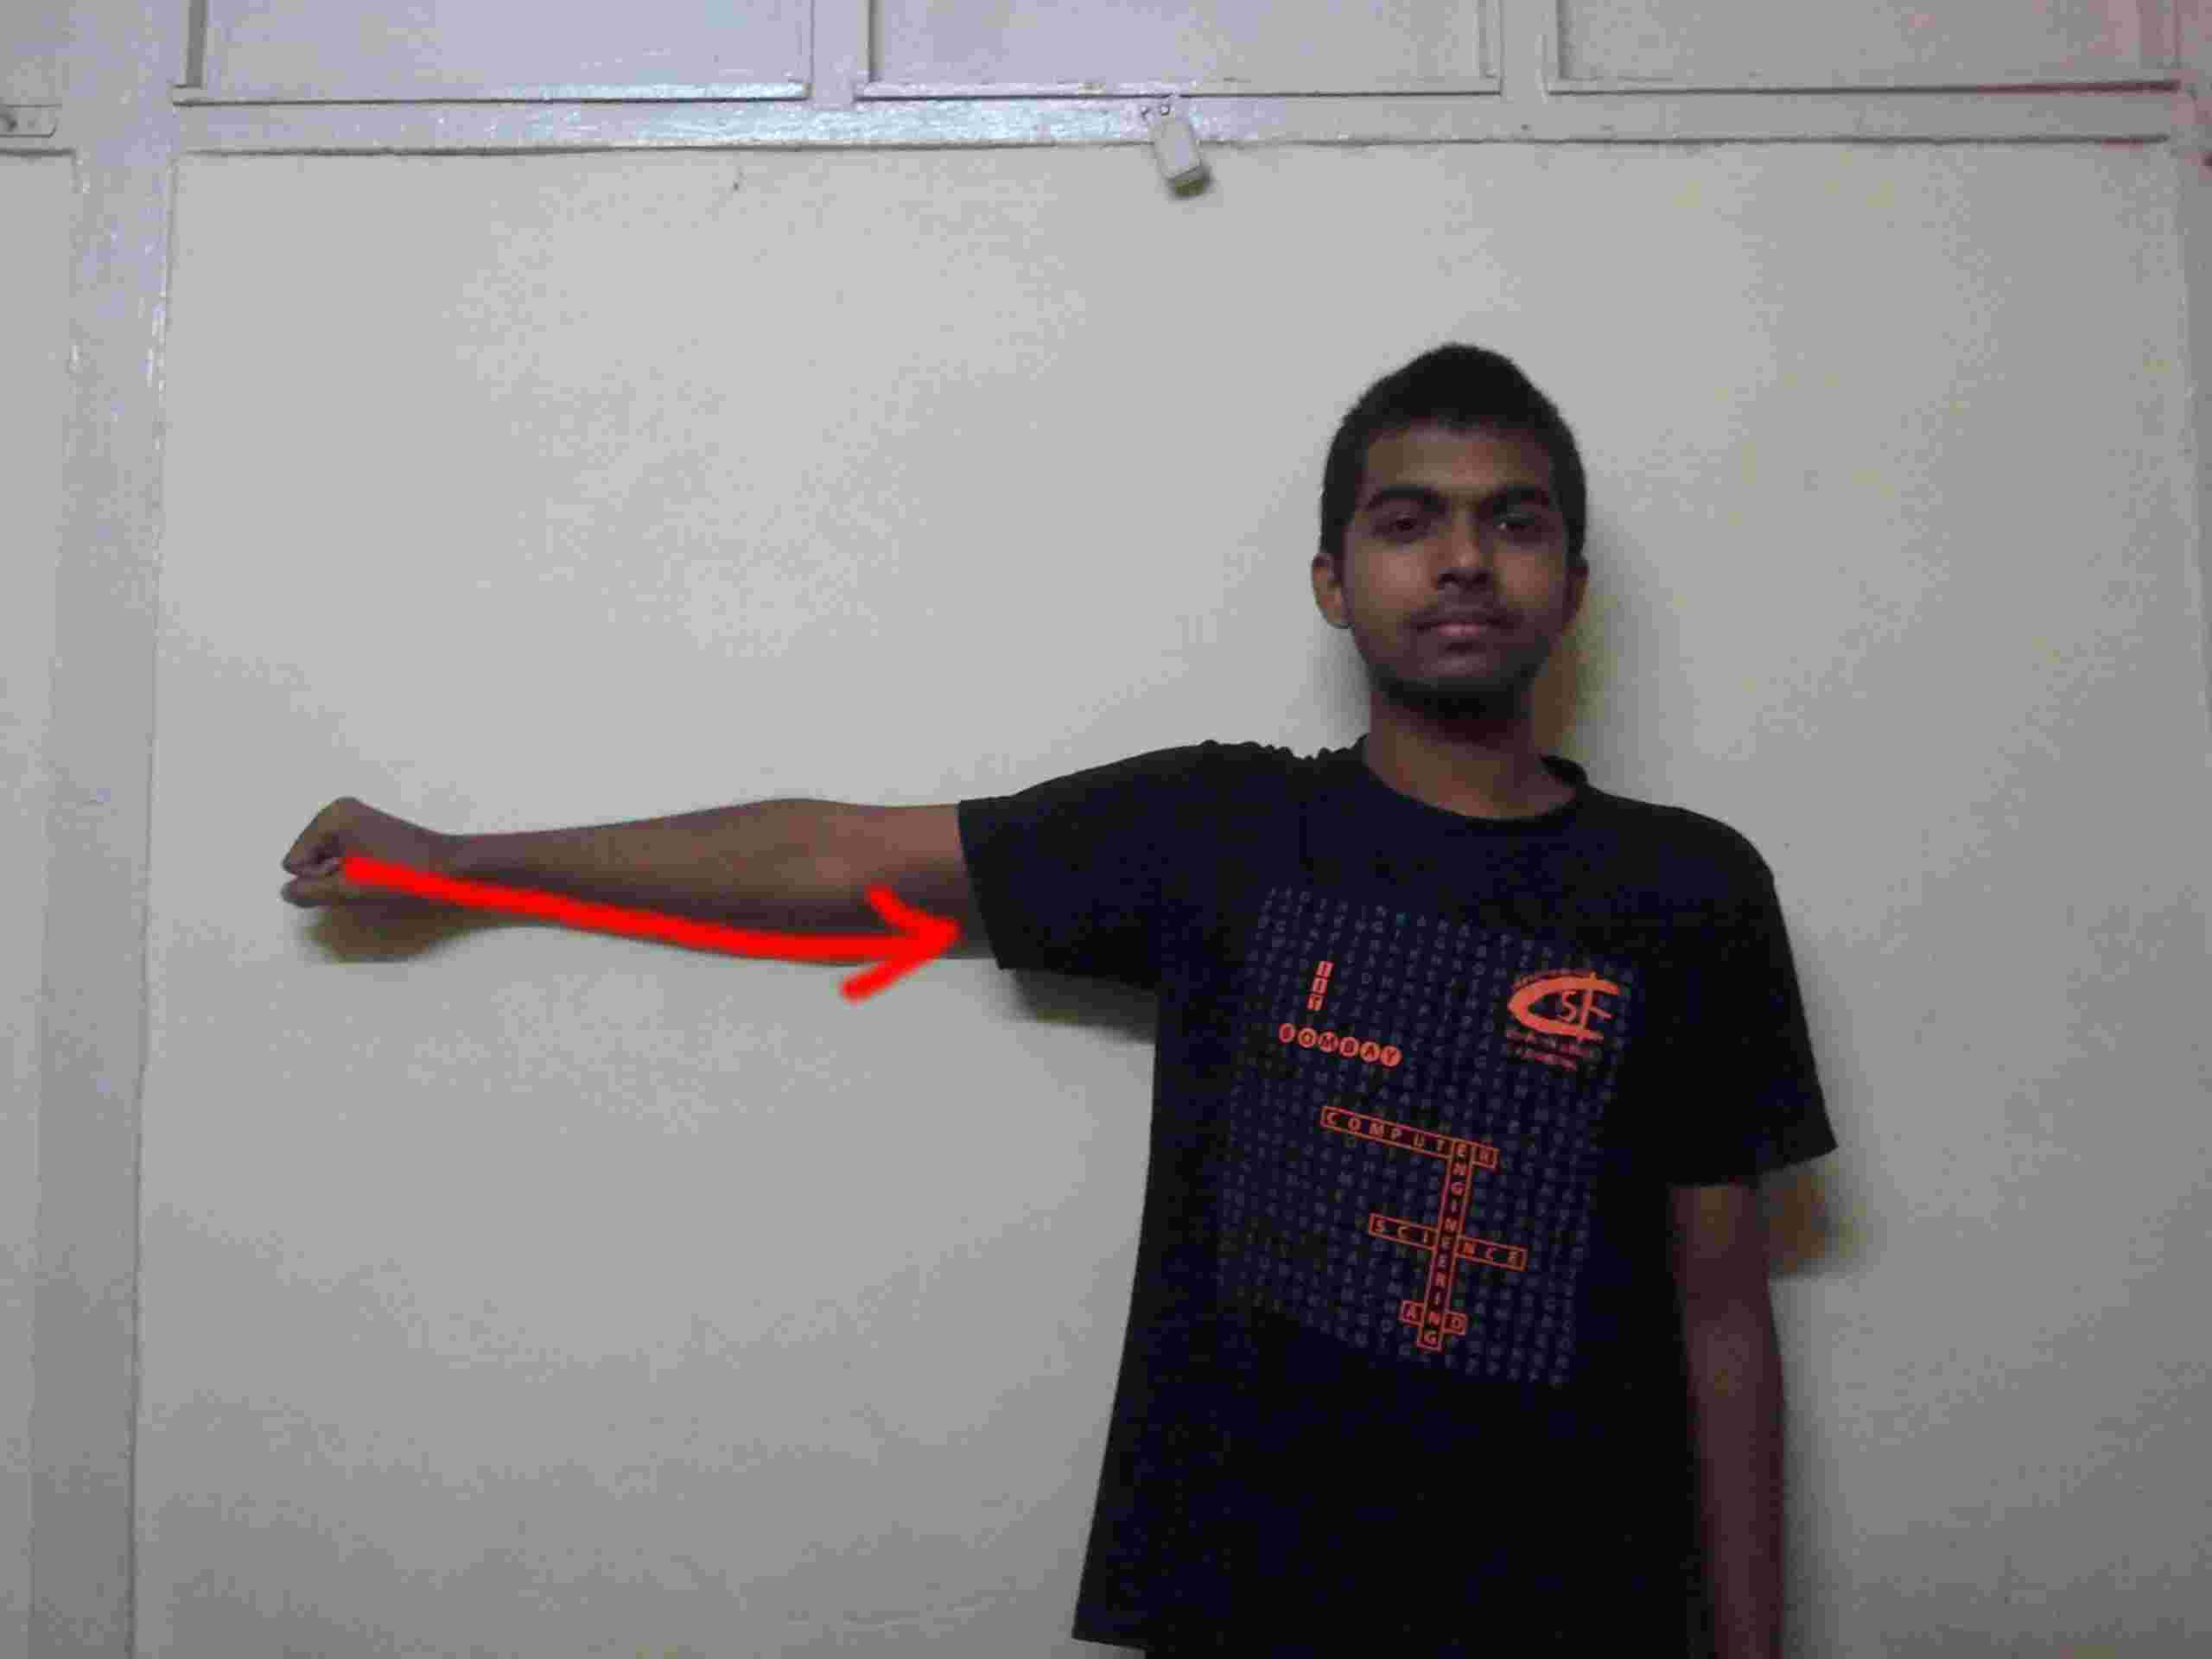
\includegraphics[scale=0.07]{gestures/11.jpg} &
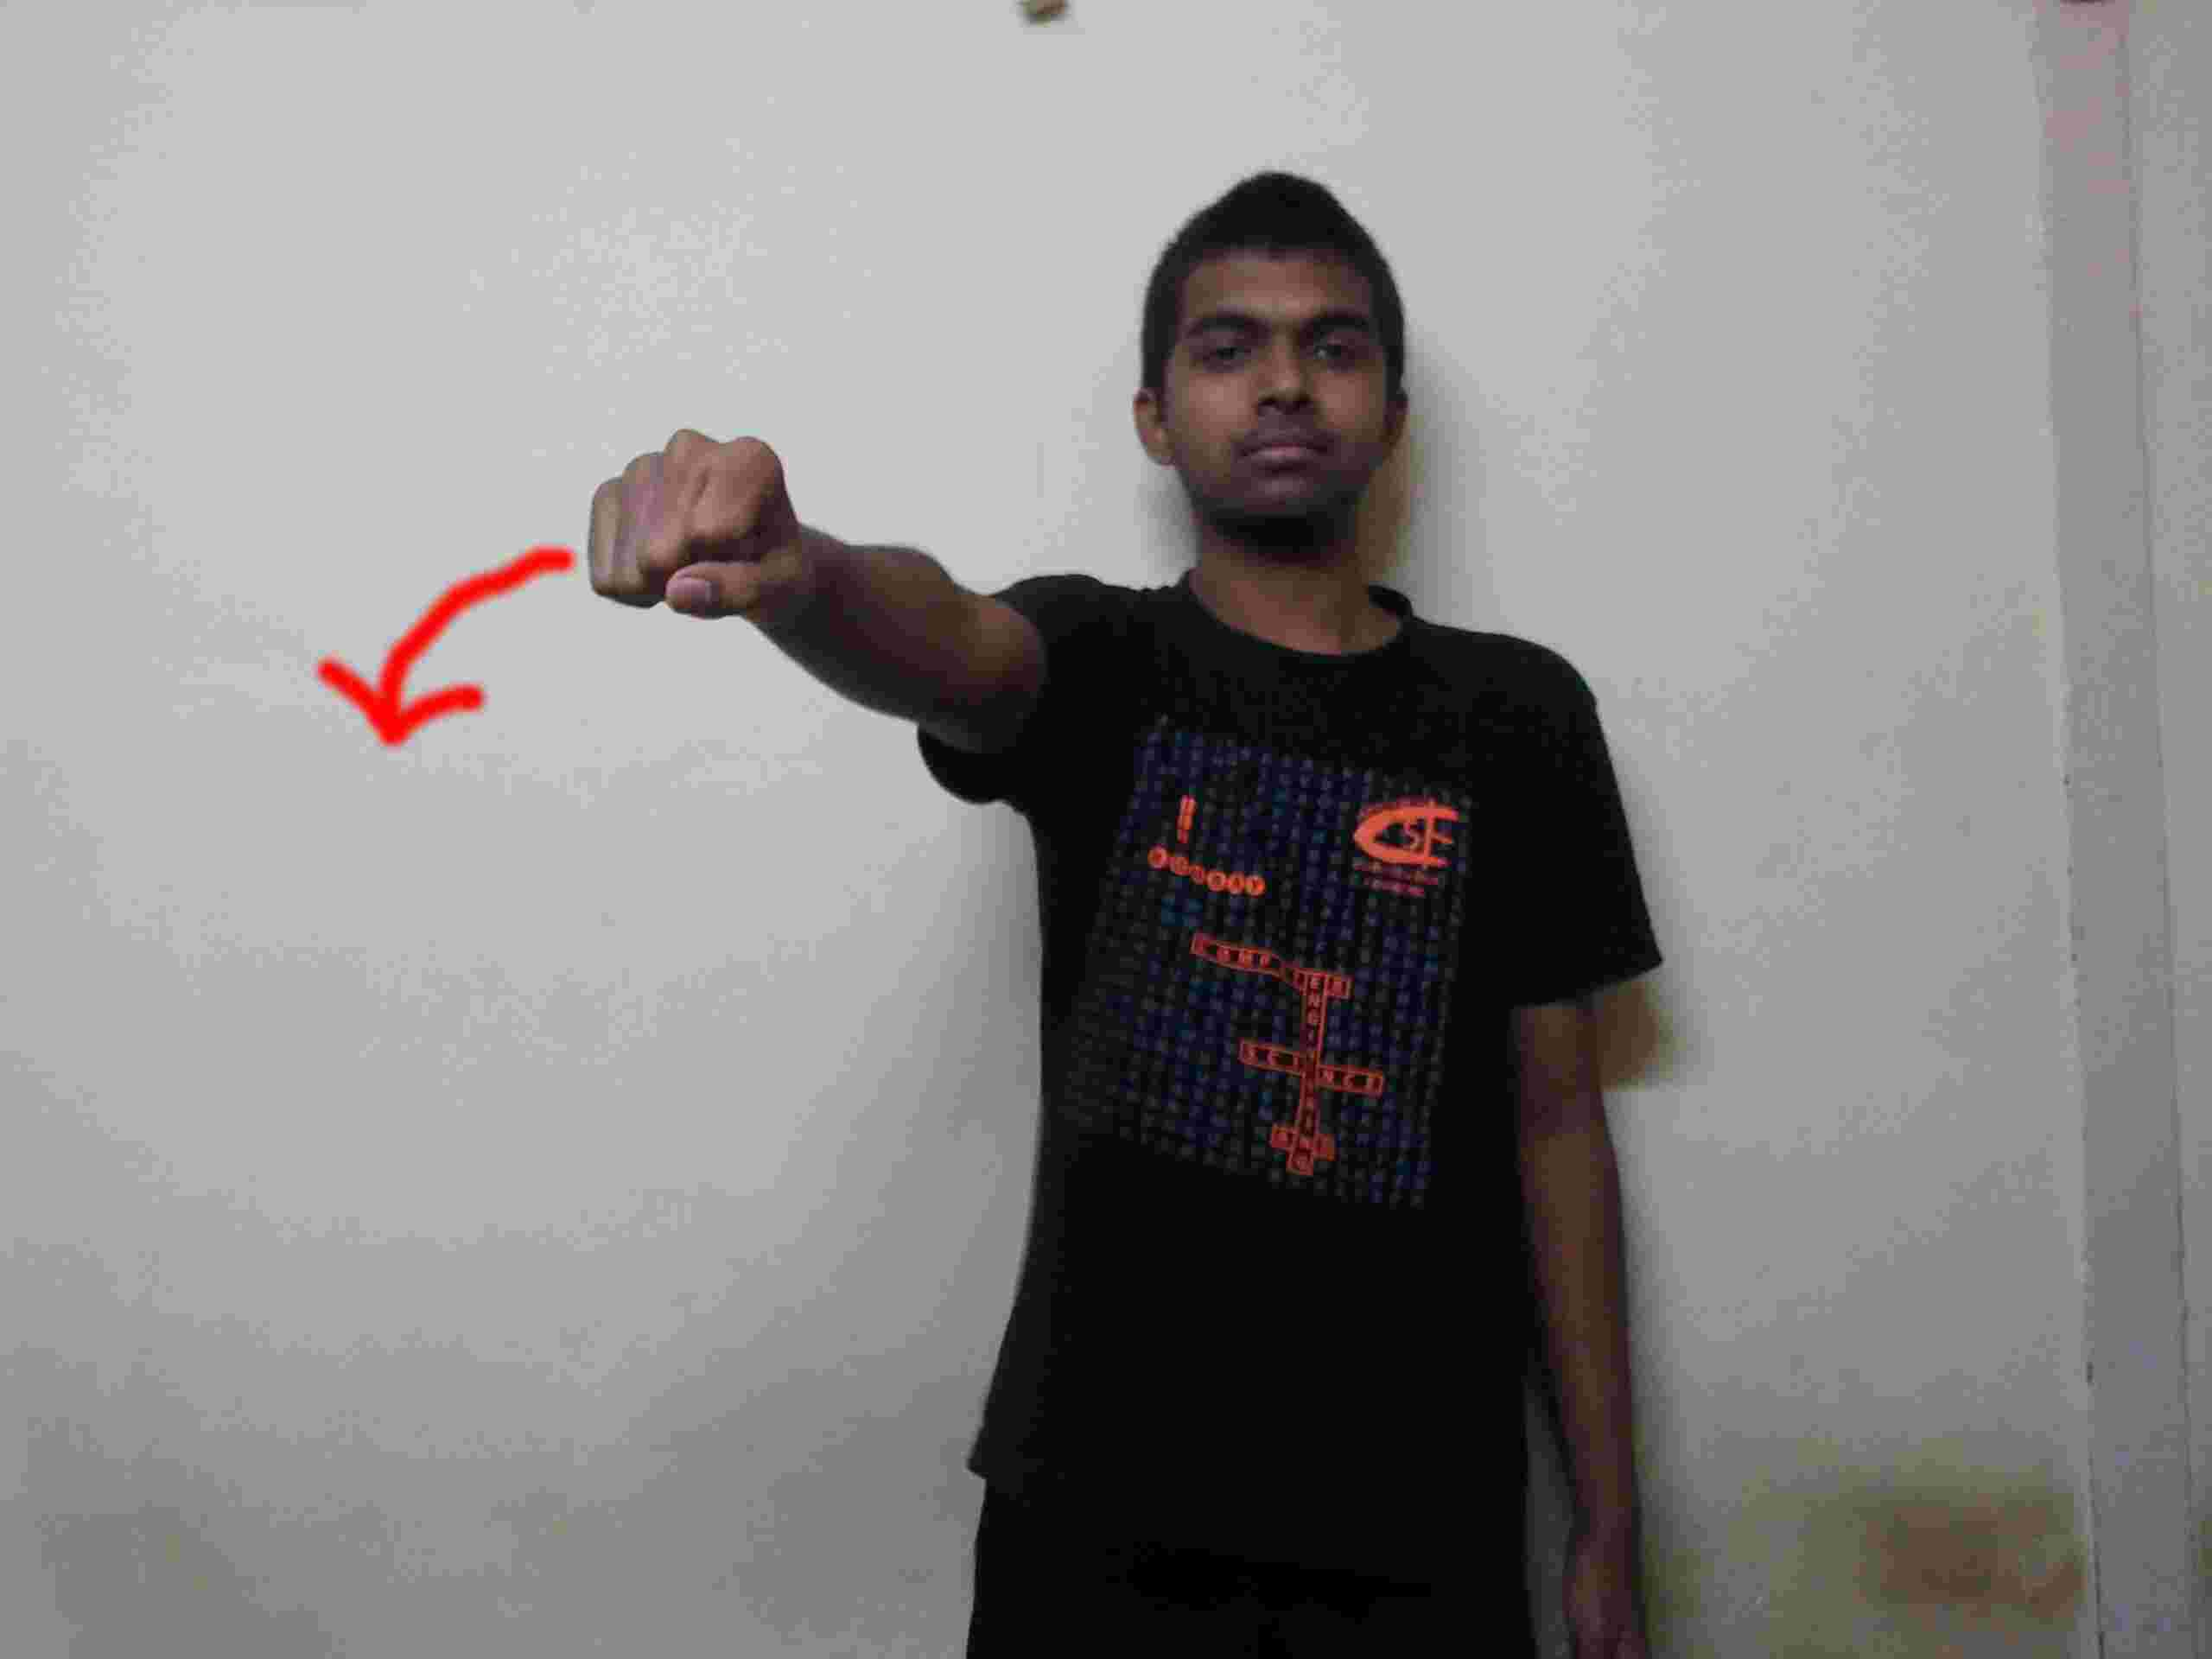
\includegraphics[scale=0.07]{gestures/12.jpg}
\end{array}
$
\end{figure}
\section*{2.Shoulder Rotation}
\begin{figure}[H]
\centering
$
\begin{array}{cc}
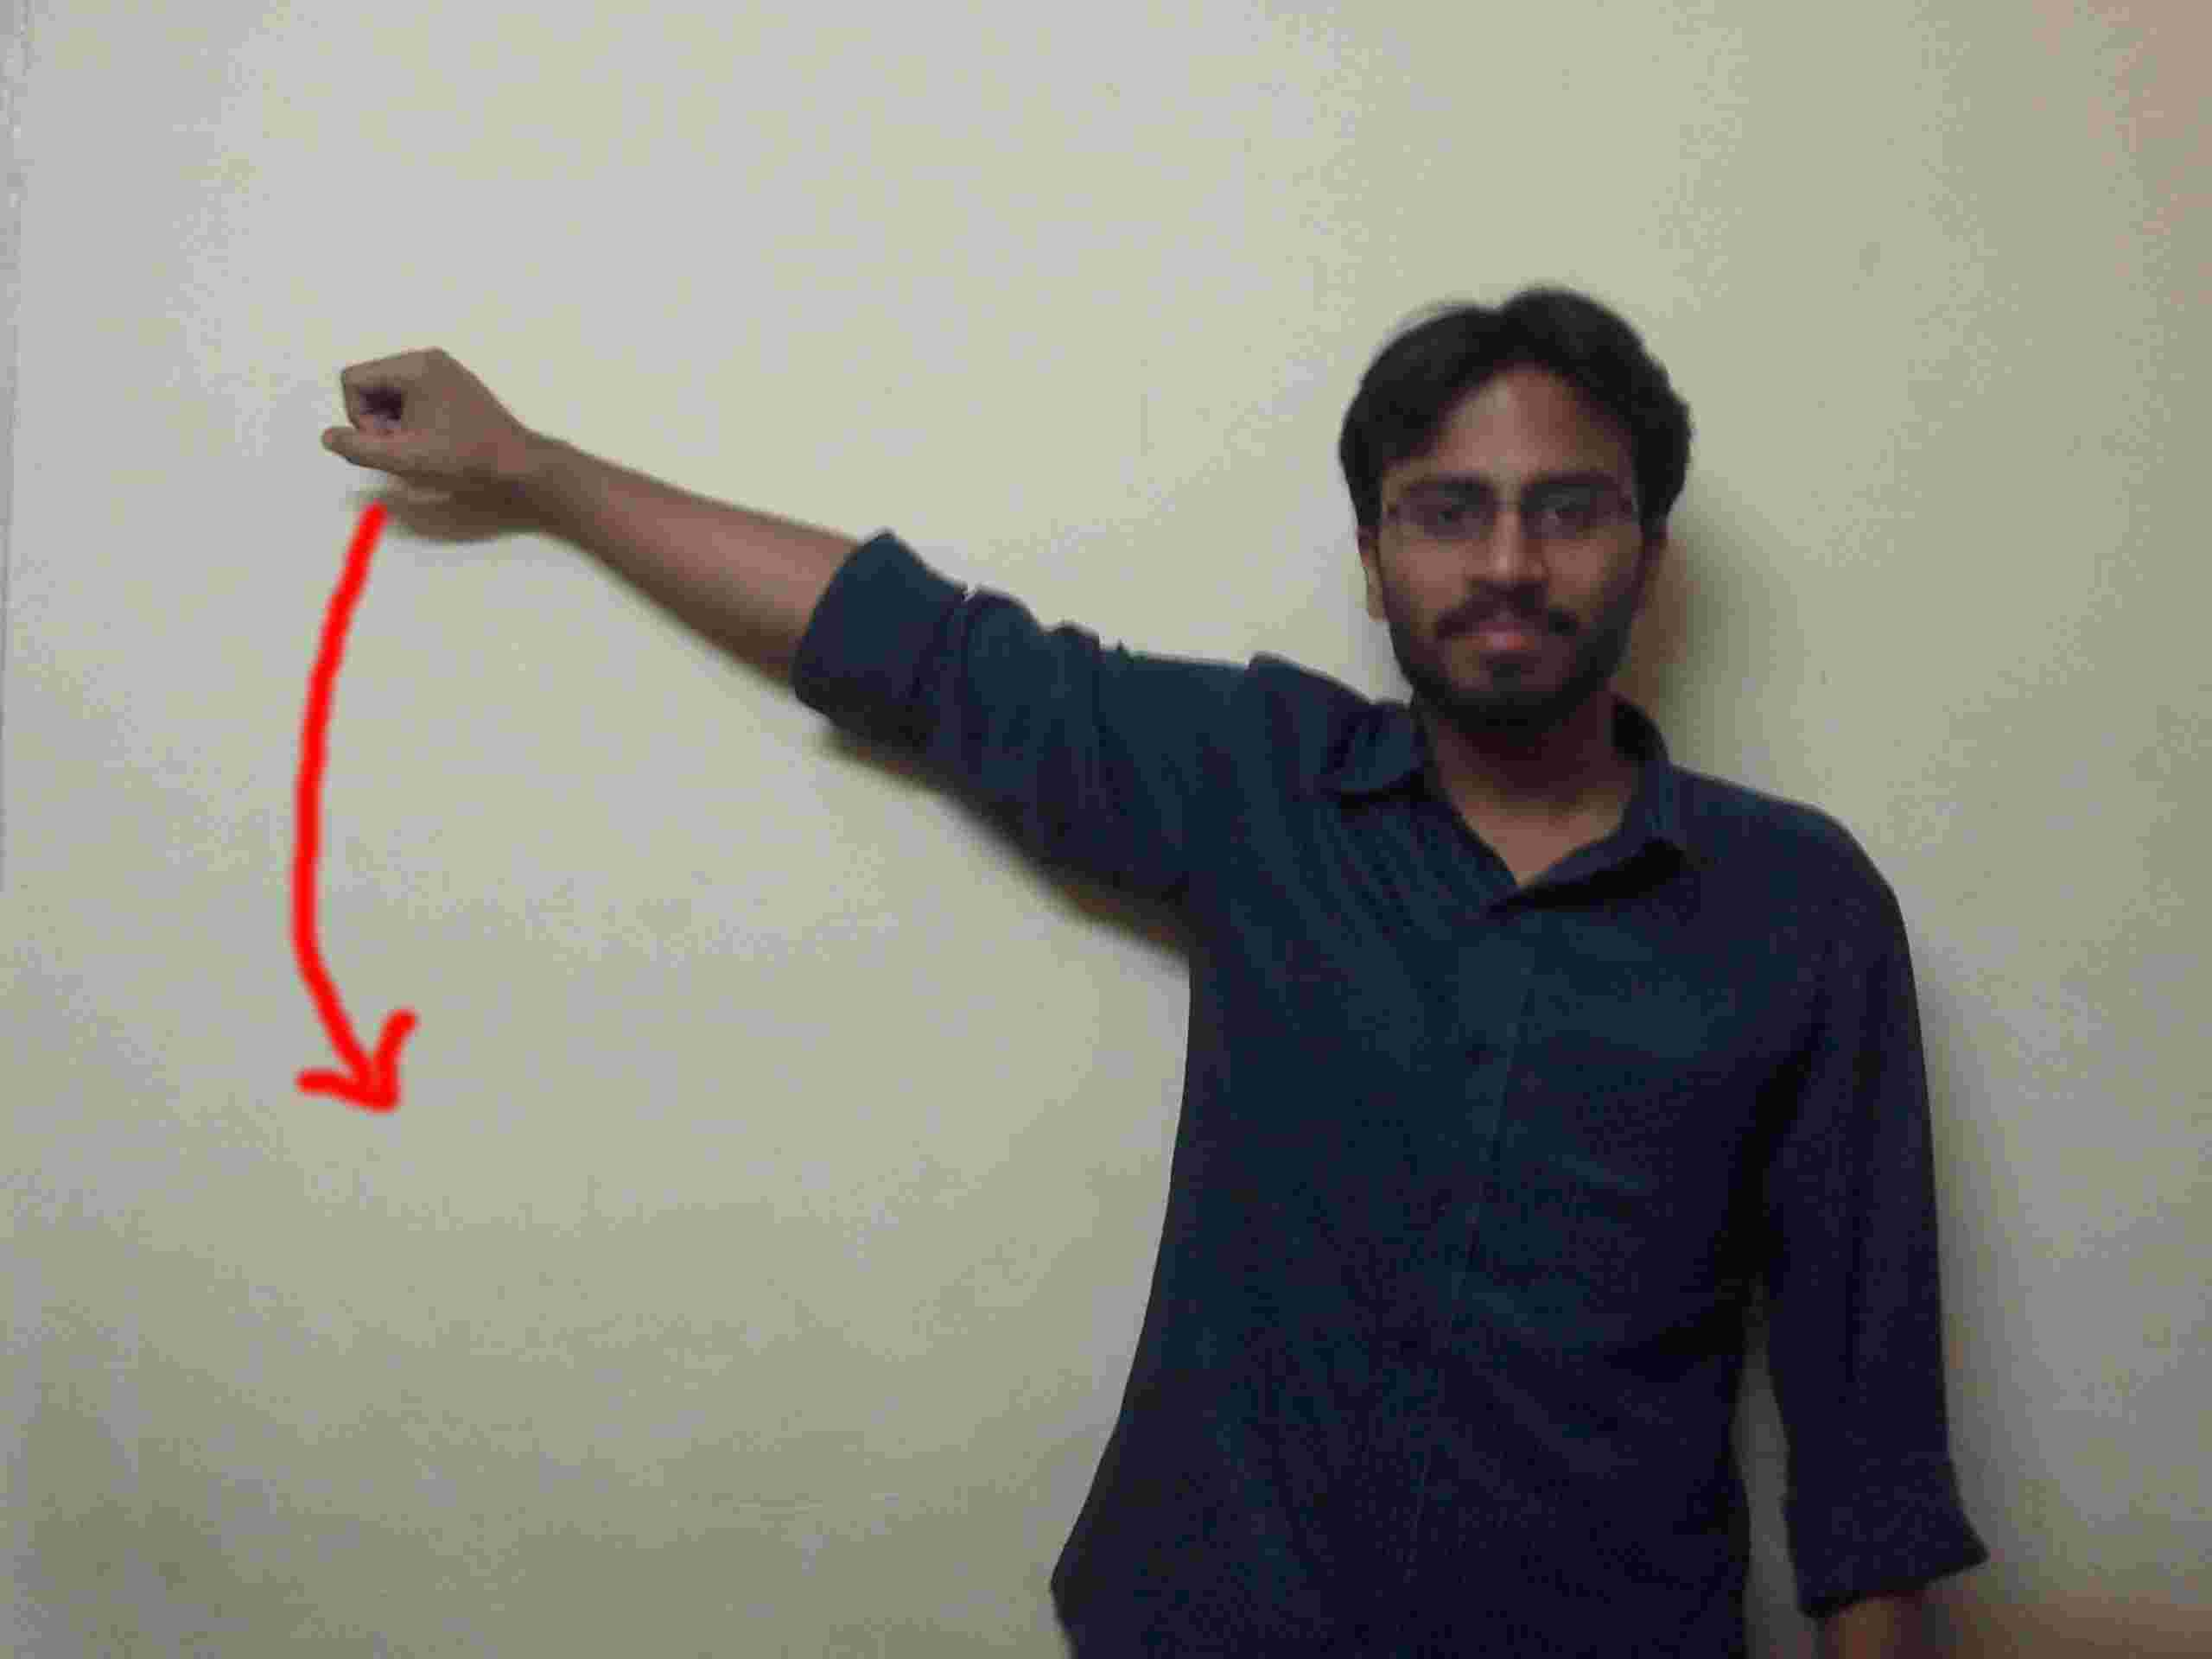
\includegraphics[scale=0.07]{gestures/21.jpg} &
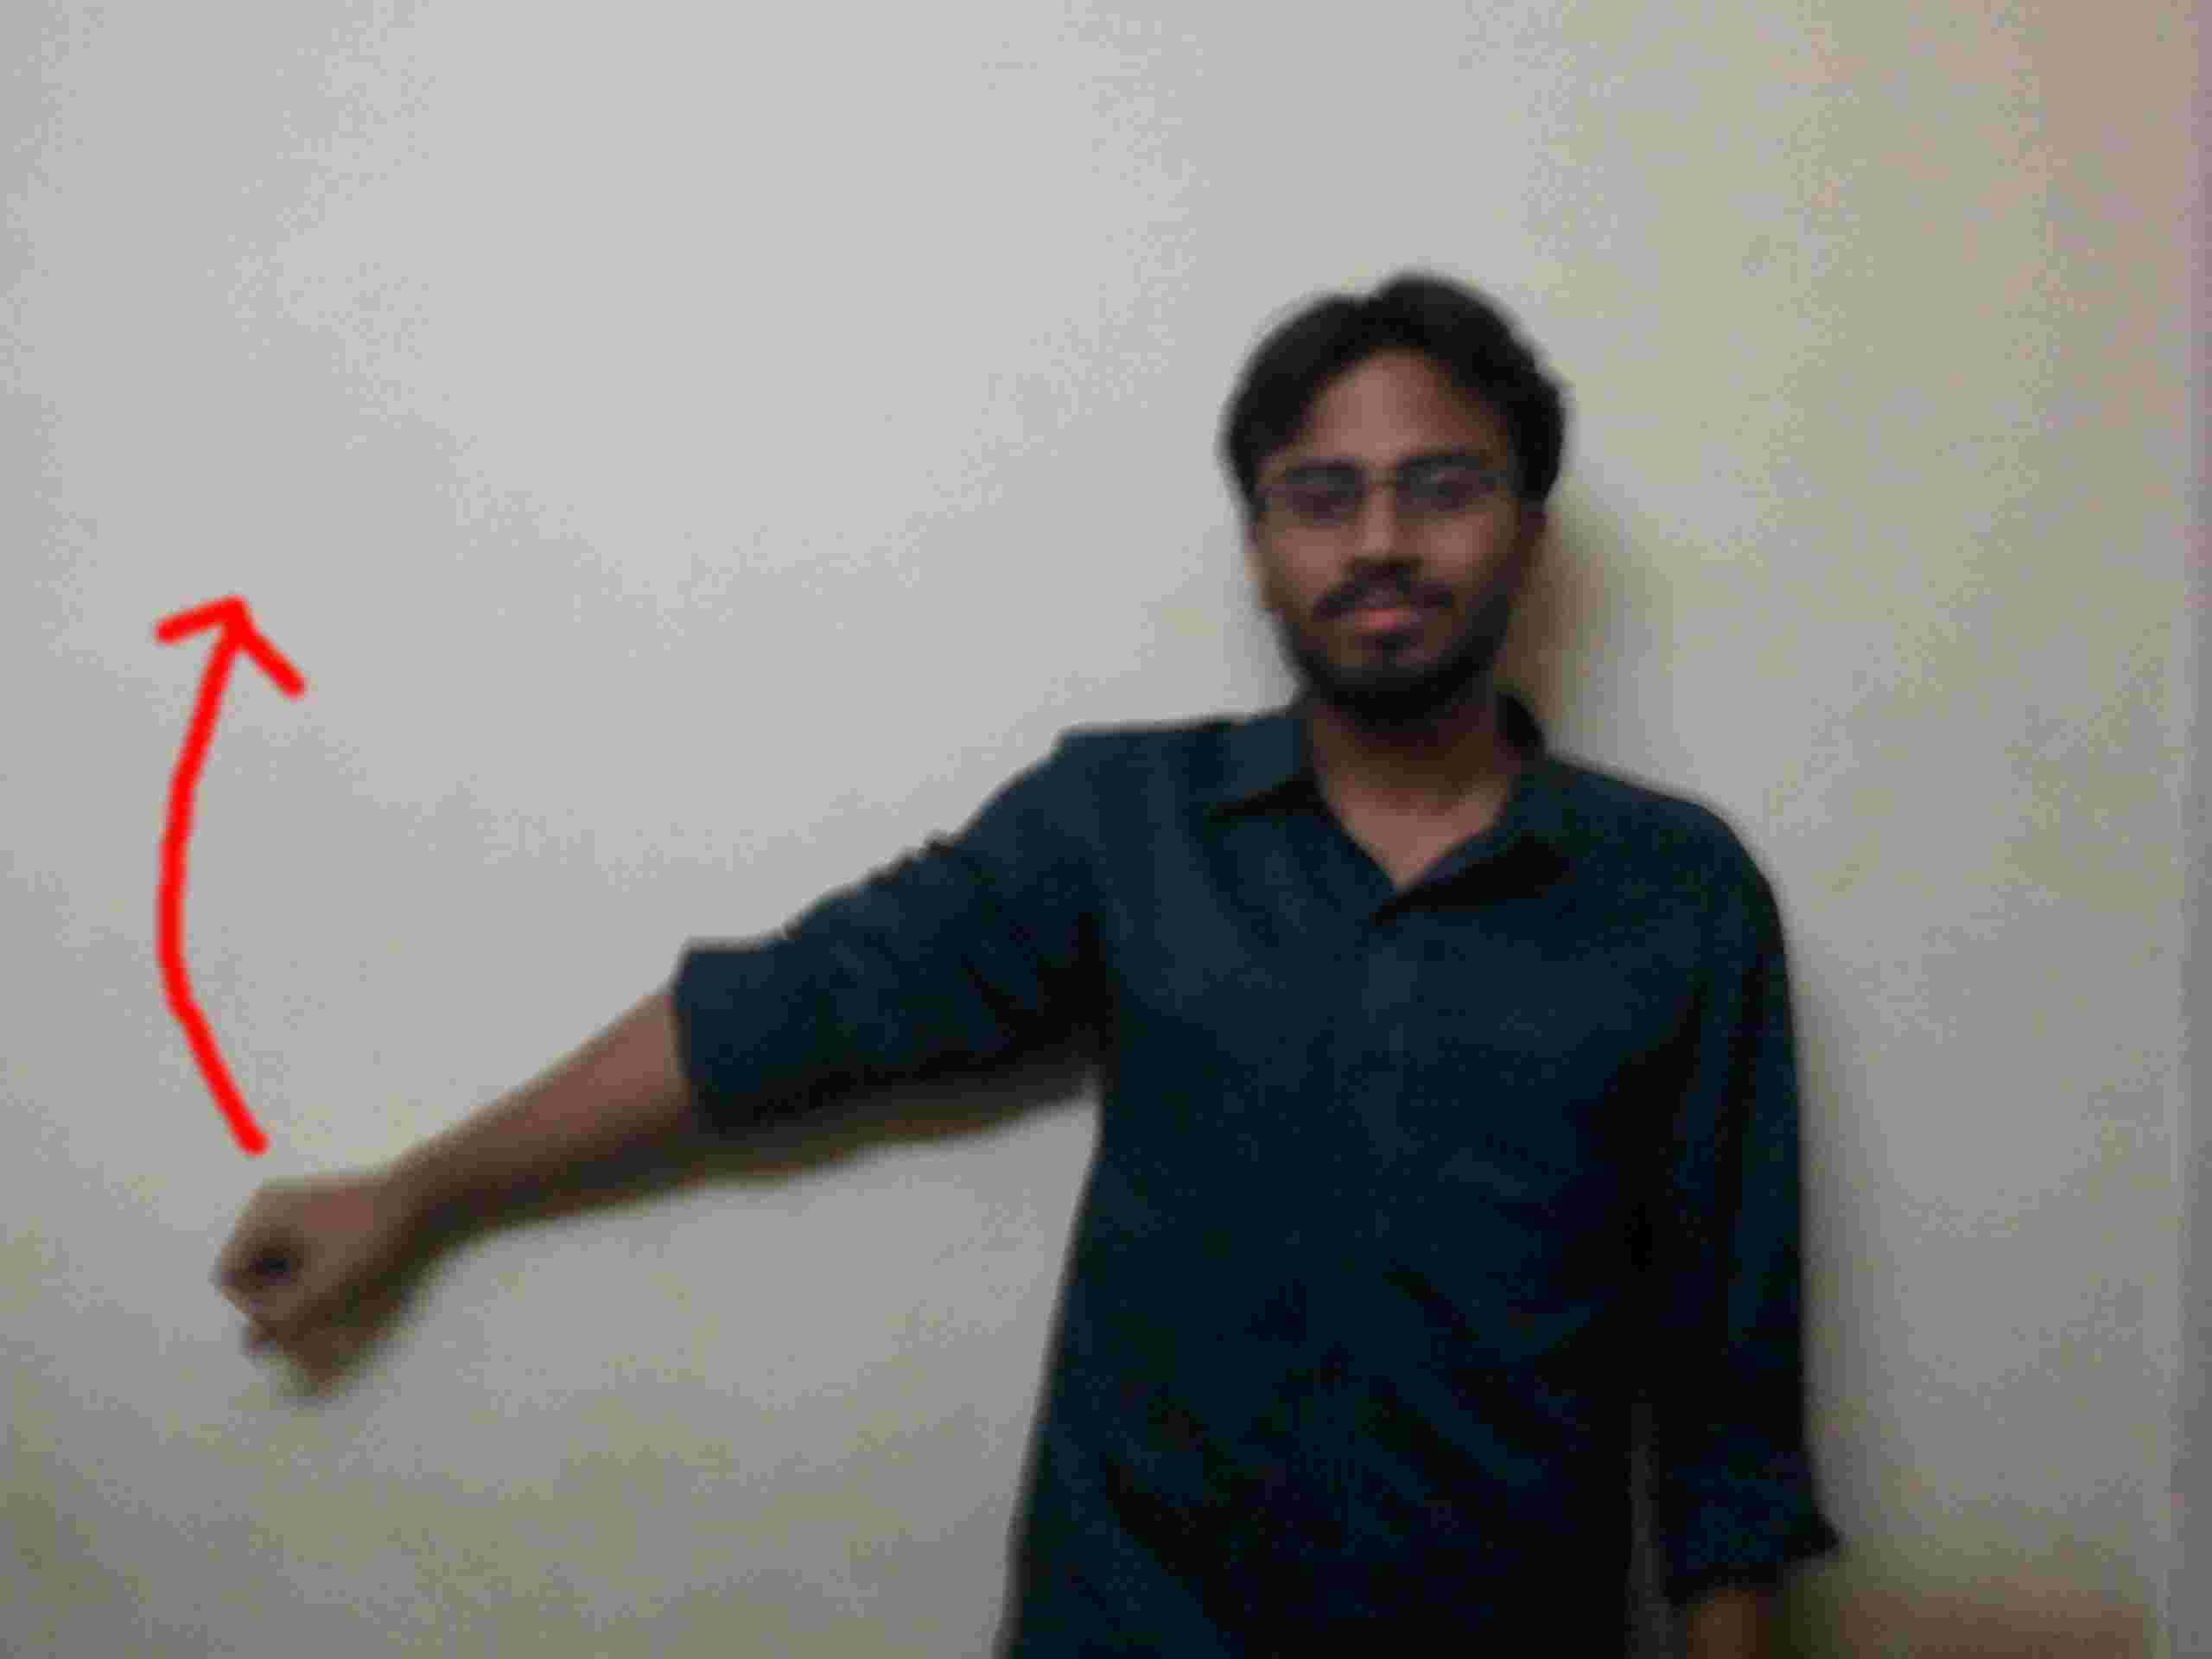
\includegraphics[scale=0.07]{gestures/22.jpg}
\end{array}
$
\end{figure}
\section*{3.Elbow Rotation}
\begin{figure}[H]
\centering
$
\begin{array}{cc}
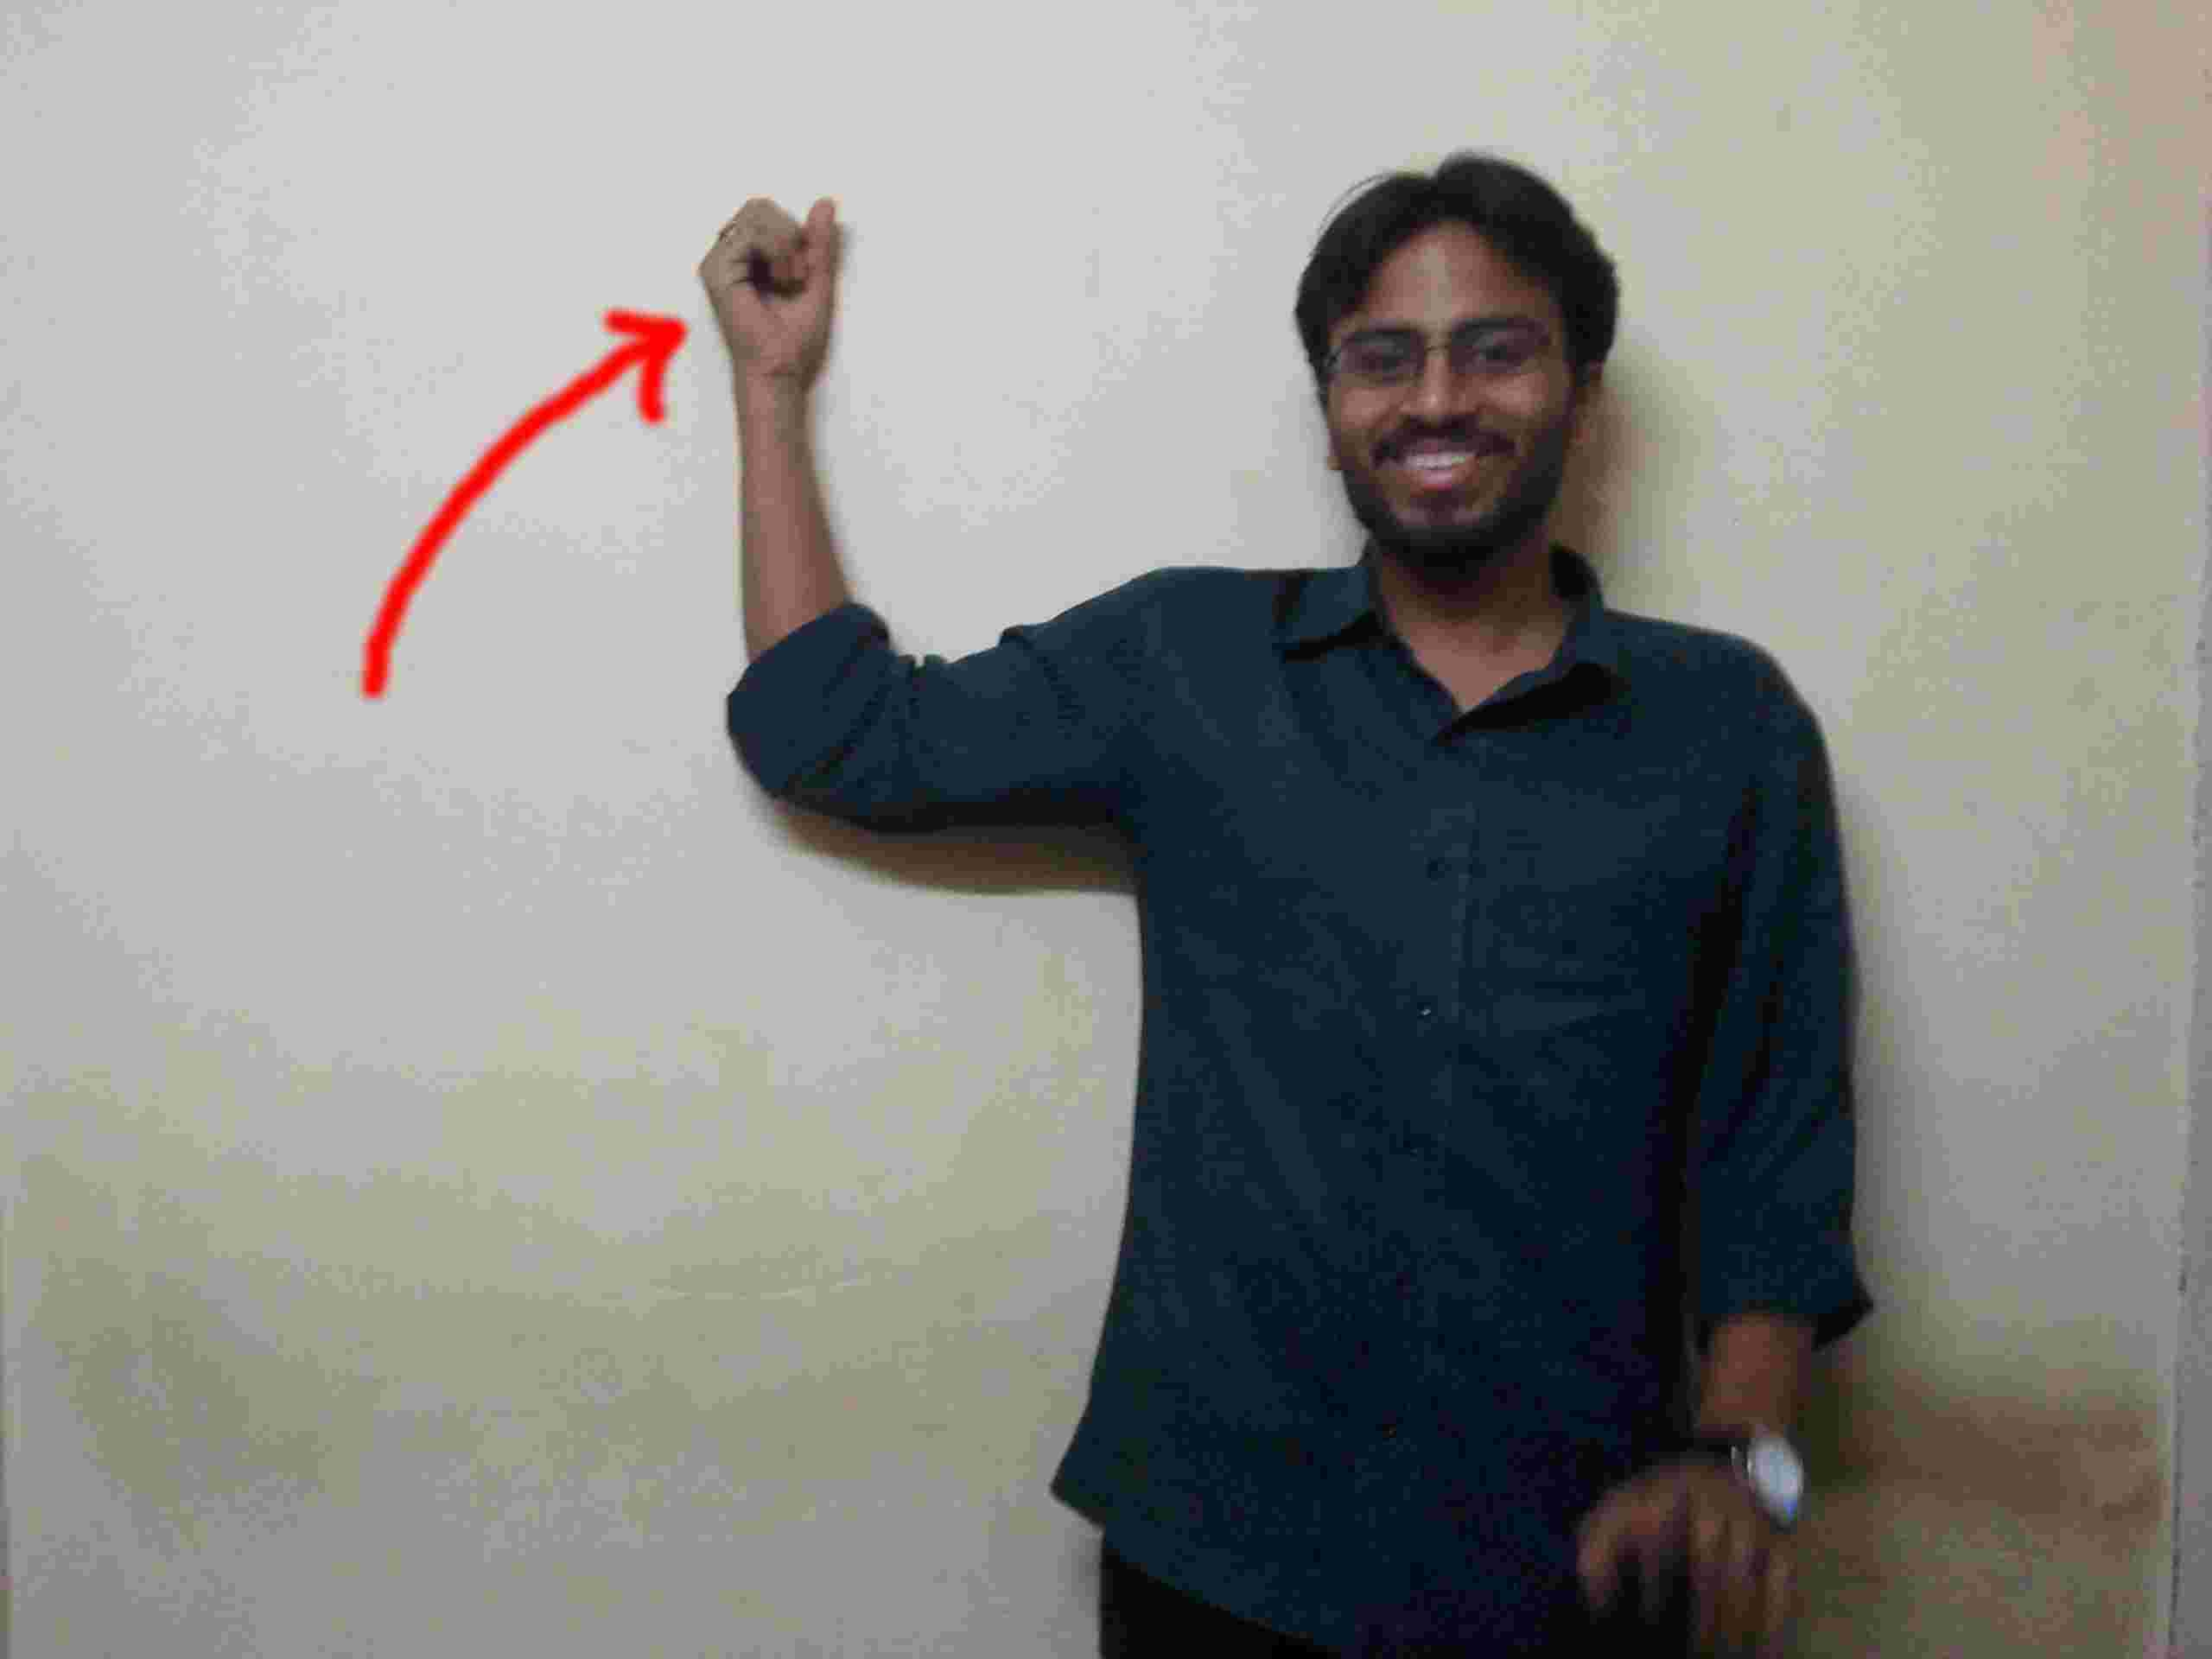
\includegraphics[scale=0.07]{gestures/31.jpg} &
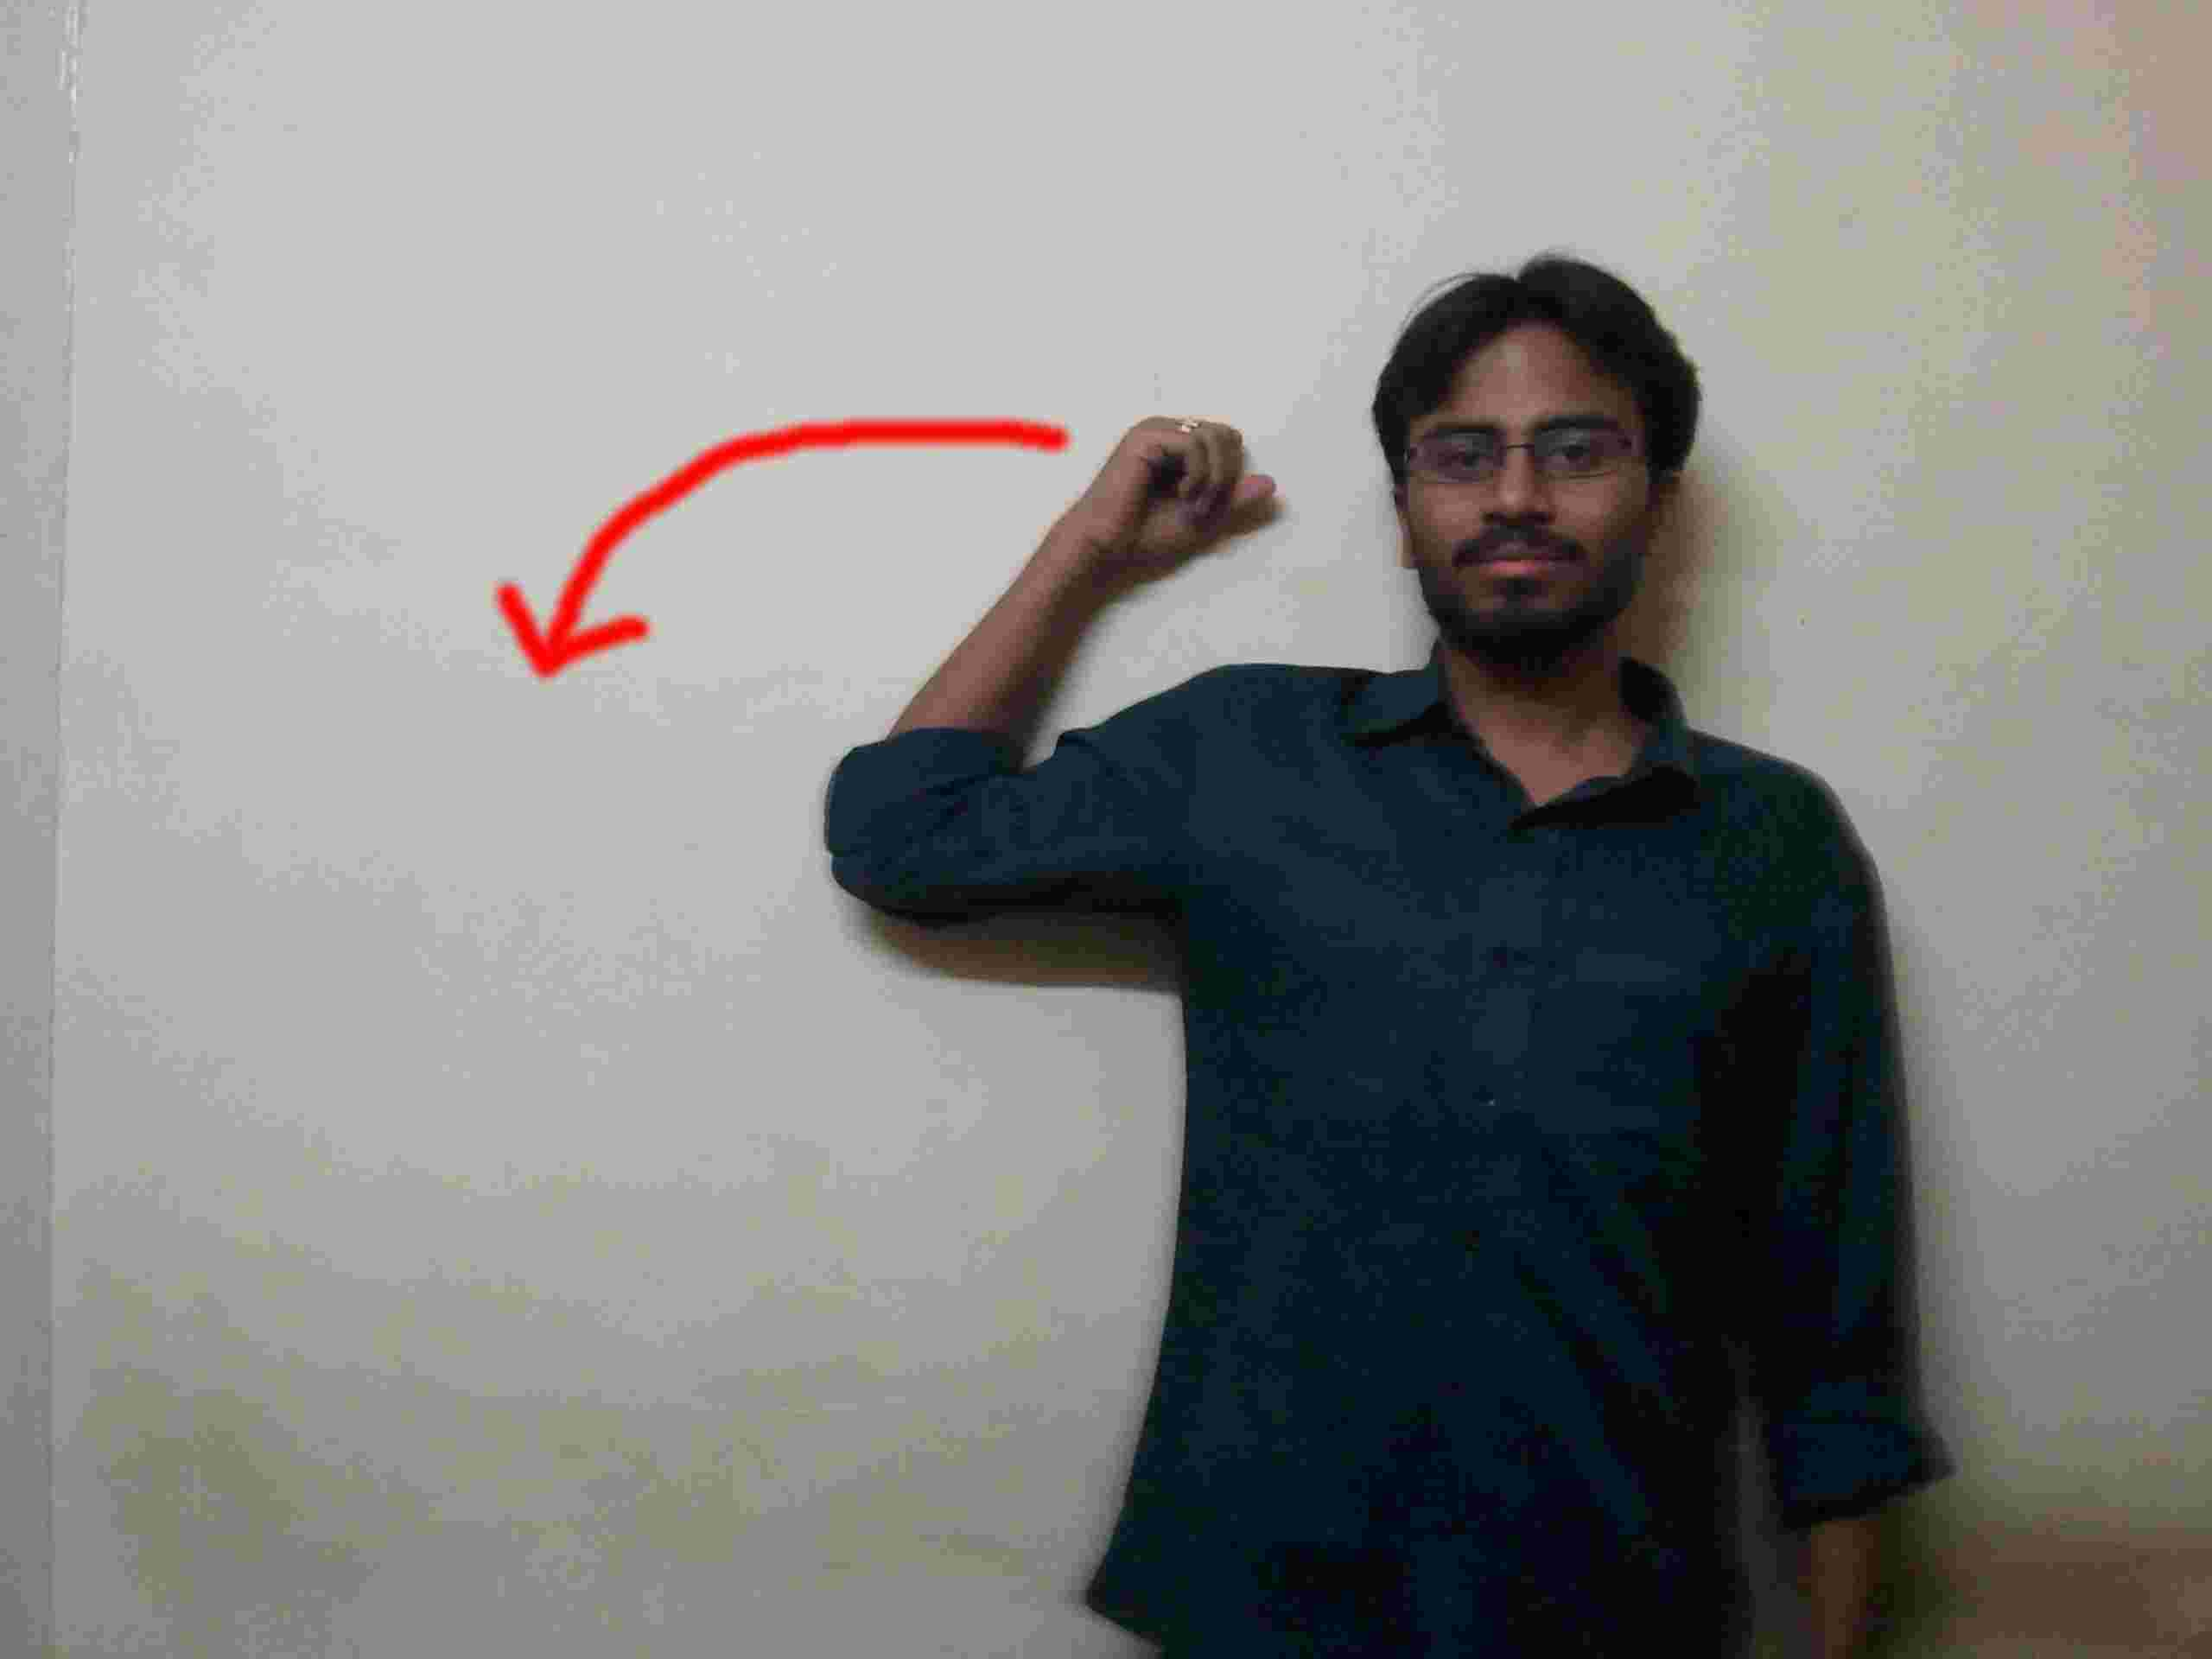
\includegraphics[scale=0.07]{gestures/32.jpg}
\end{array}
$
\end{figure}
\section*{4.Wrist Pitch}
\begin{figure}[H]
\centering
$
\begin{array}{cc}
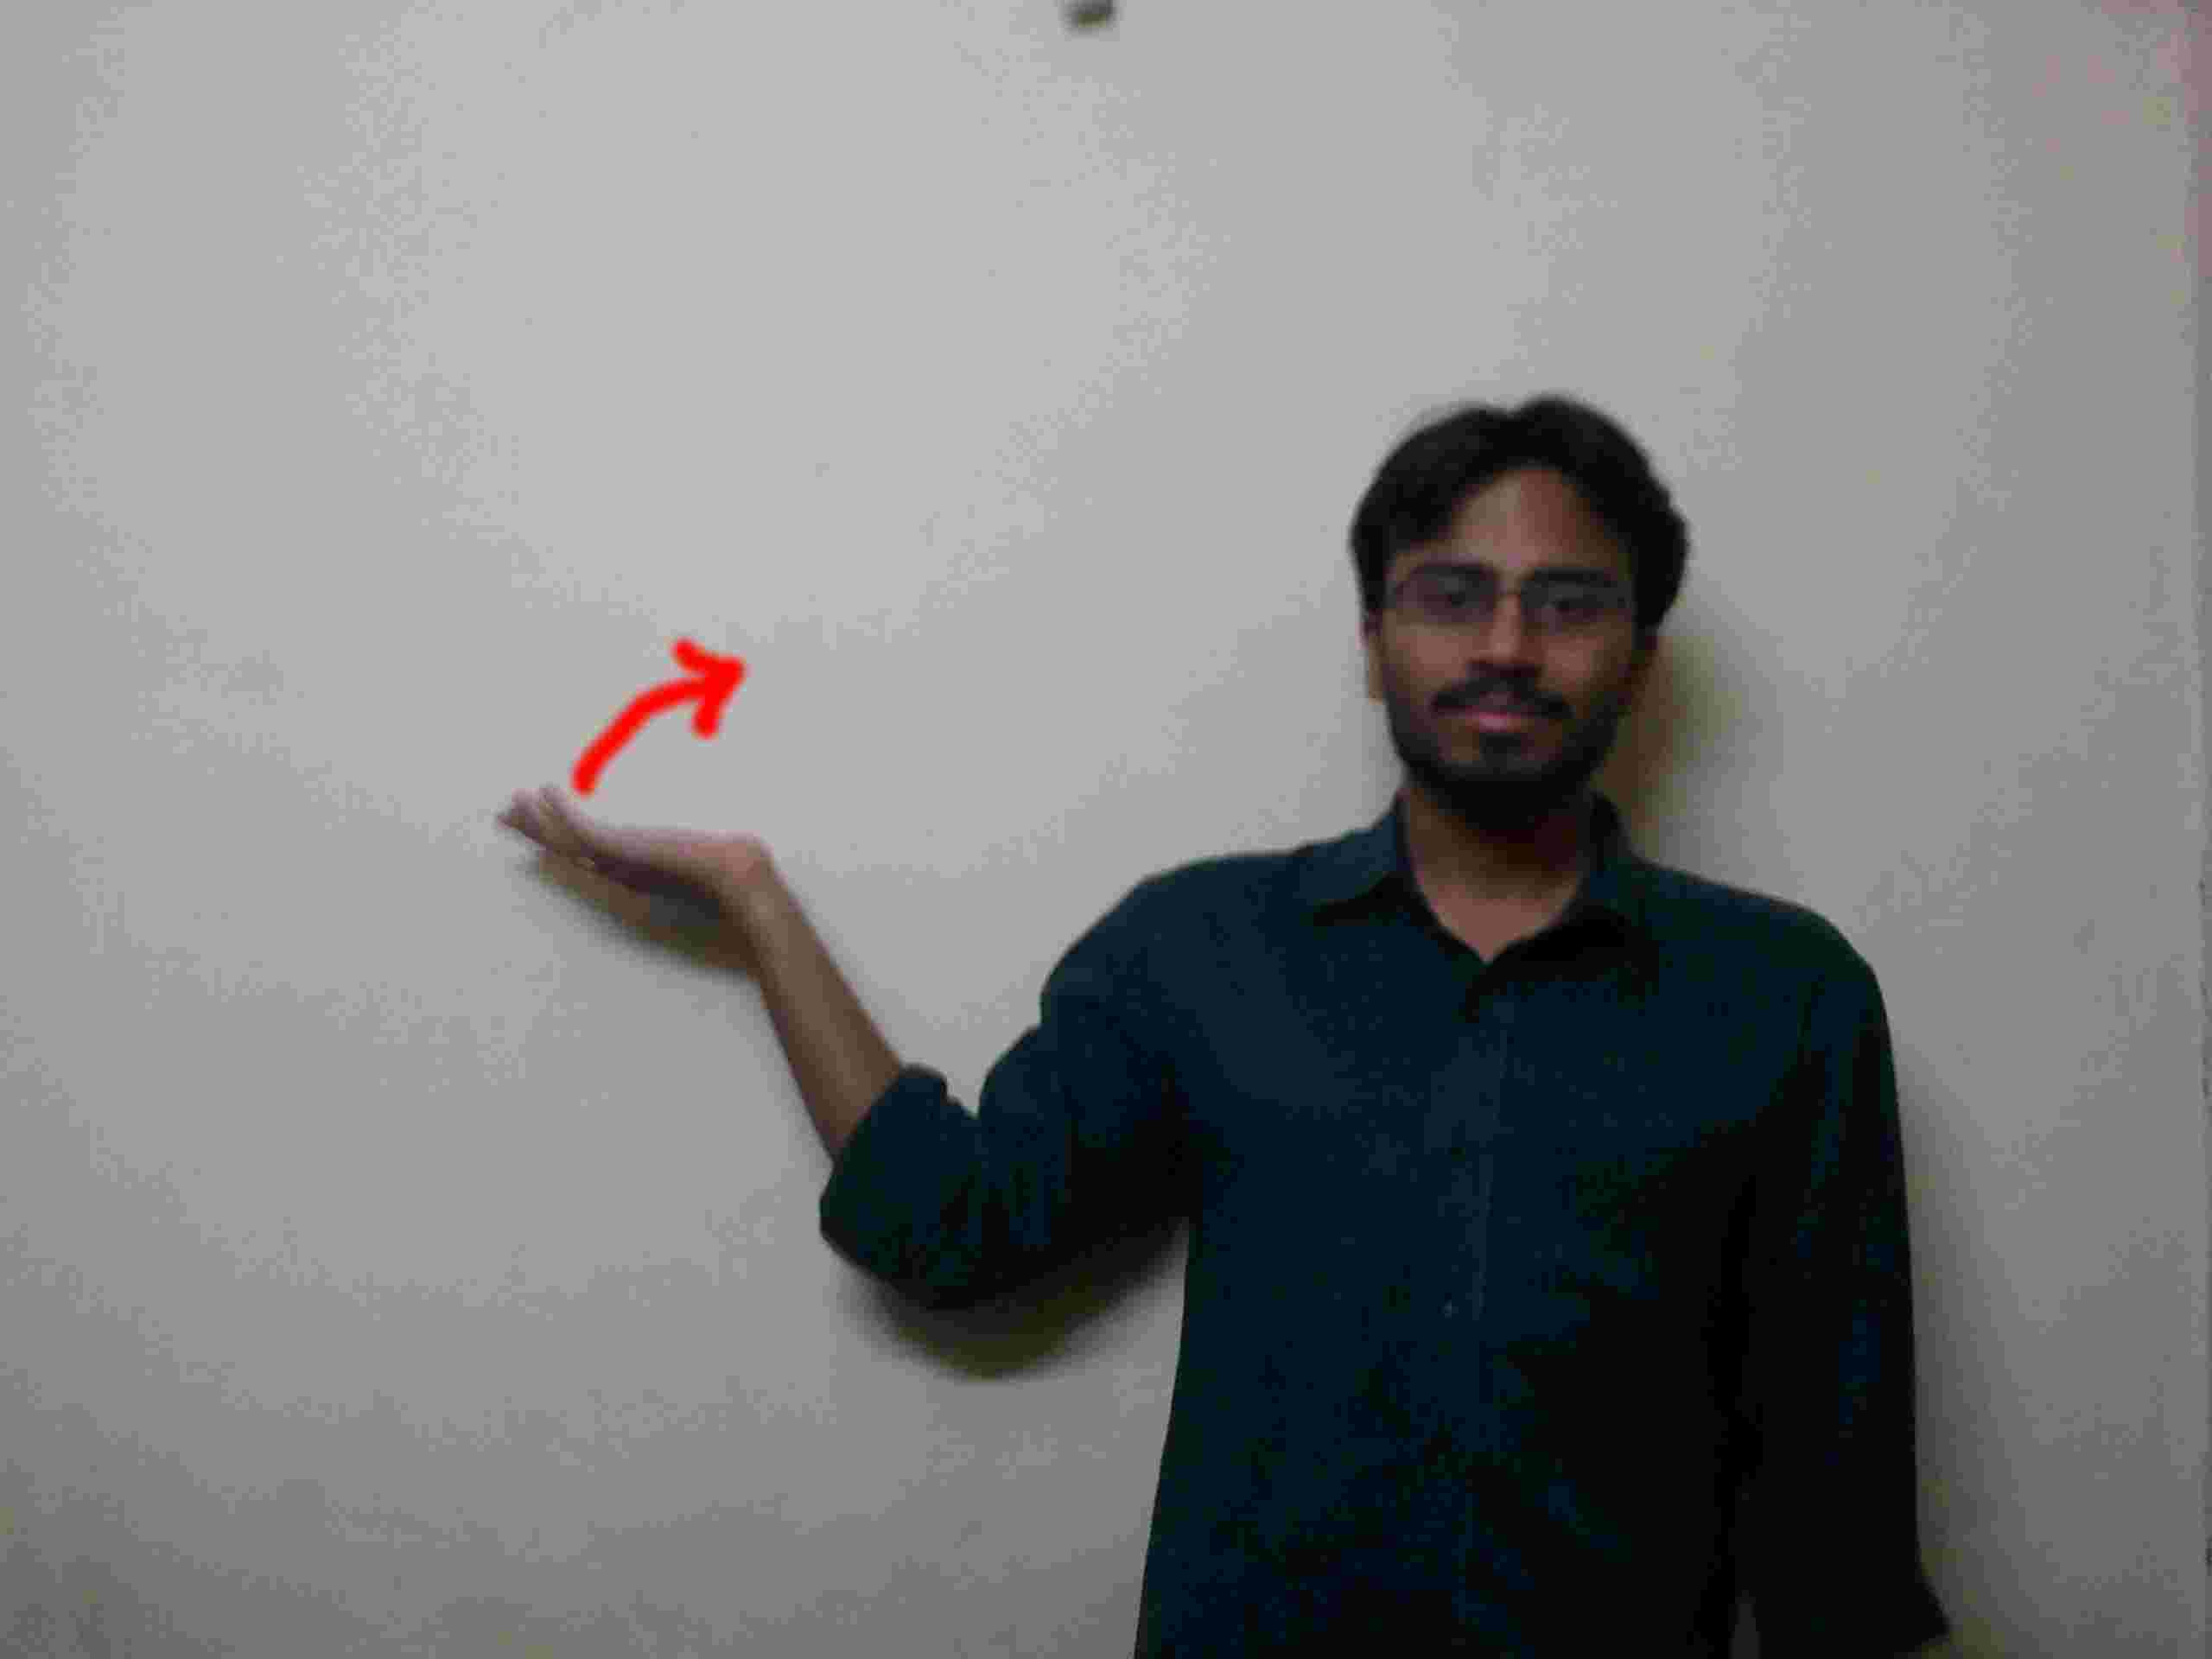
\includegraphics[scale=0.07]{gestures/41.jpg} &
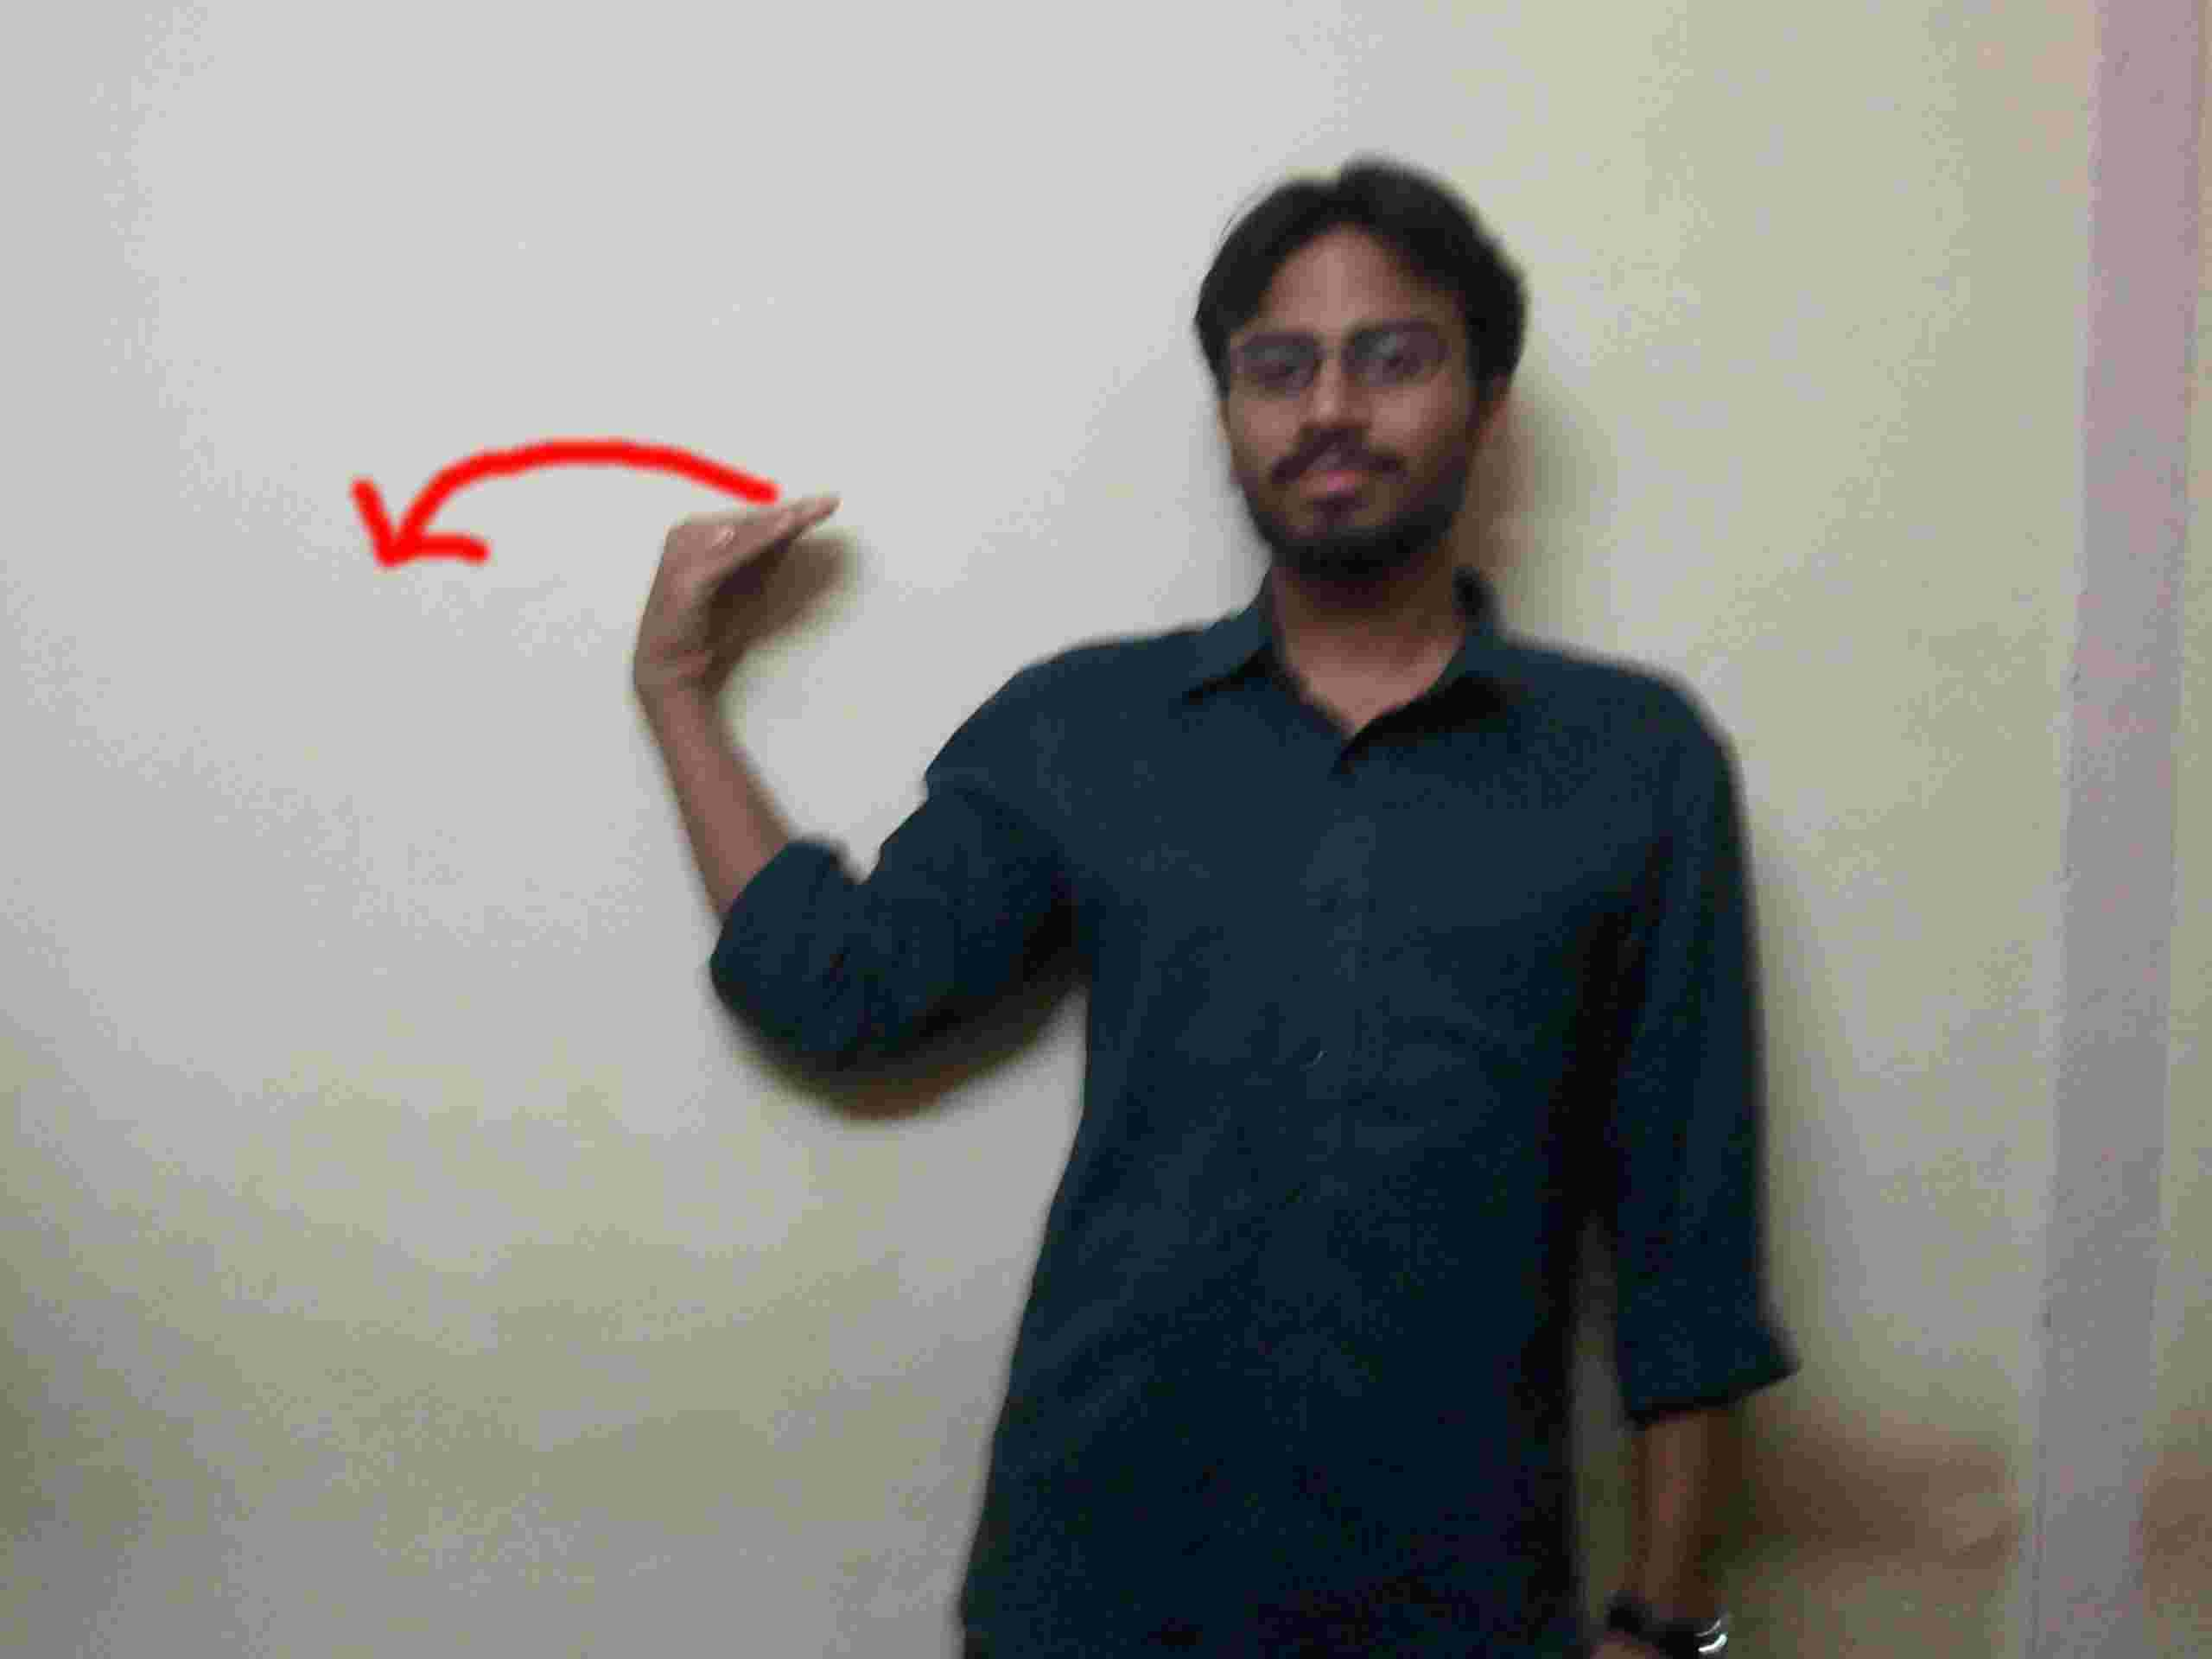
\includegraphics[scale=0.07]{gestures/42.jpg}
\end{array}
$
\end{figure}
\section*{5.Wrist Roll}
\begin{figure}[H]
\centering
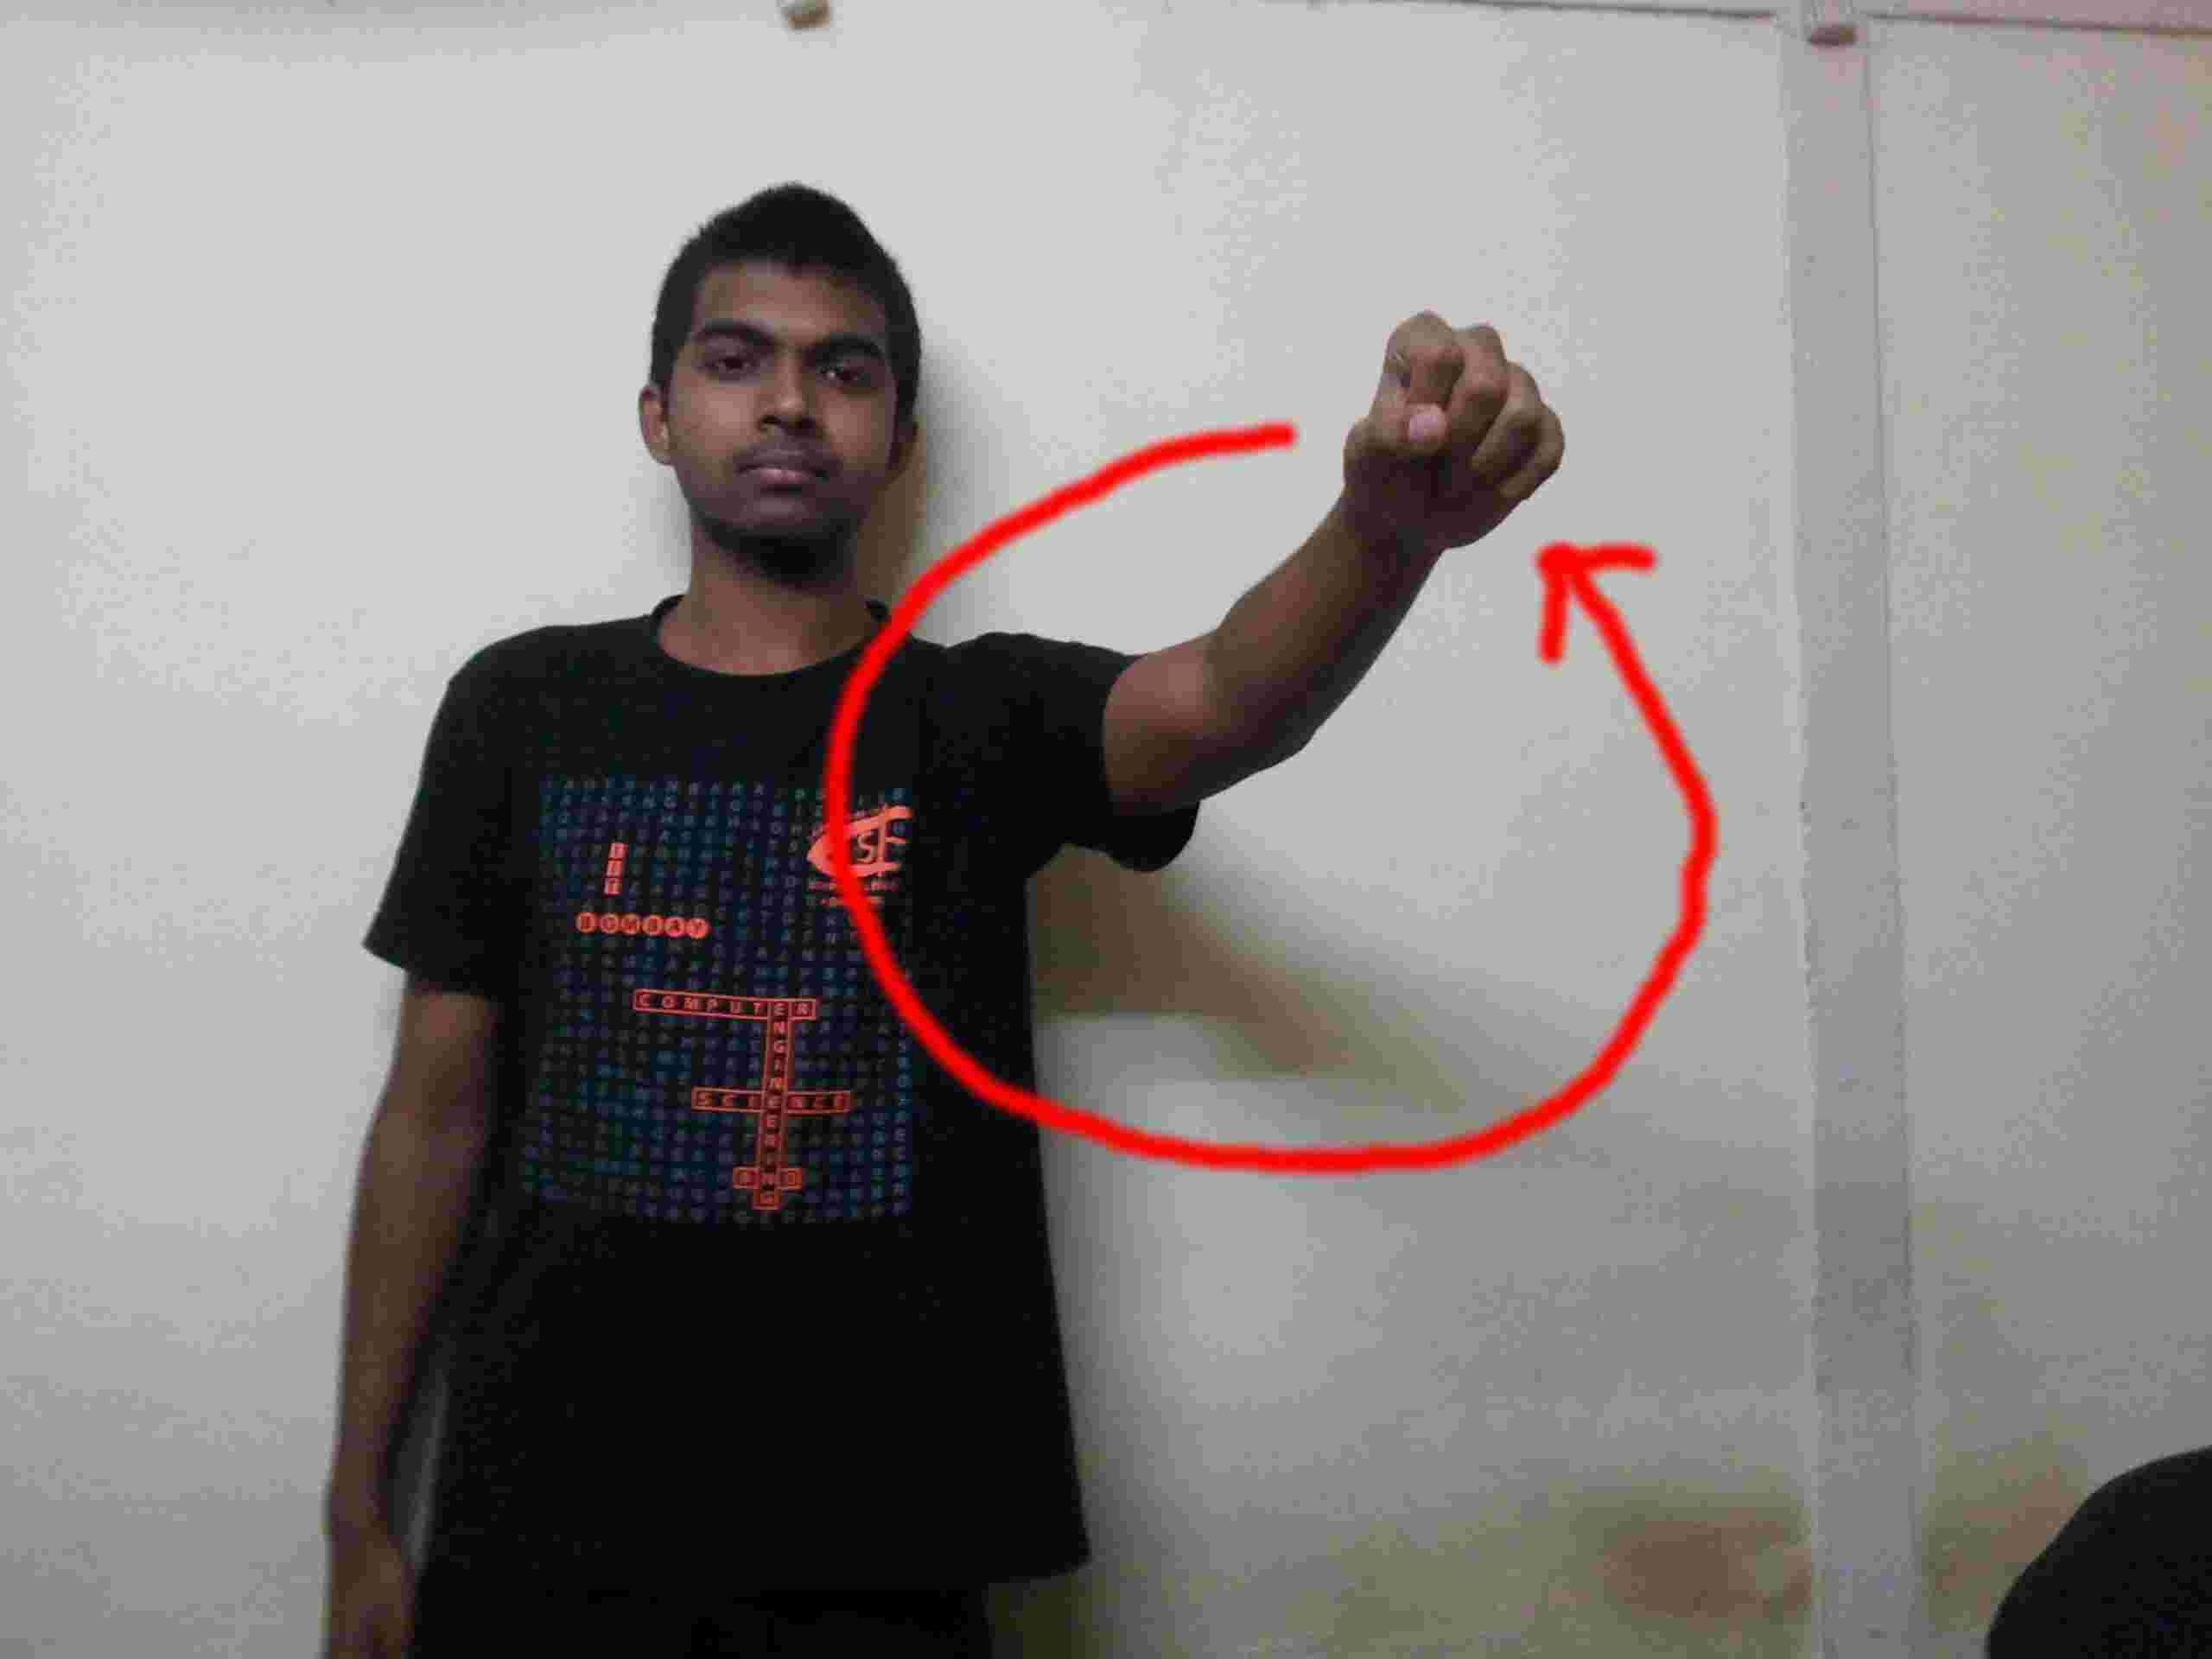
\includegraphics[scale=0.1]{gestures/5.jpg}
\end{figure}
\section*{6.Grip and Ungrip}
\begin{figure}[H]
\centering
$
\begin{array}{cc}
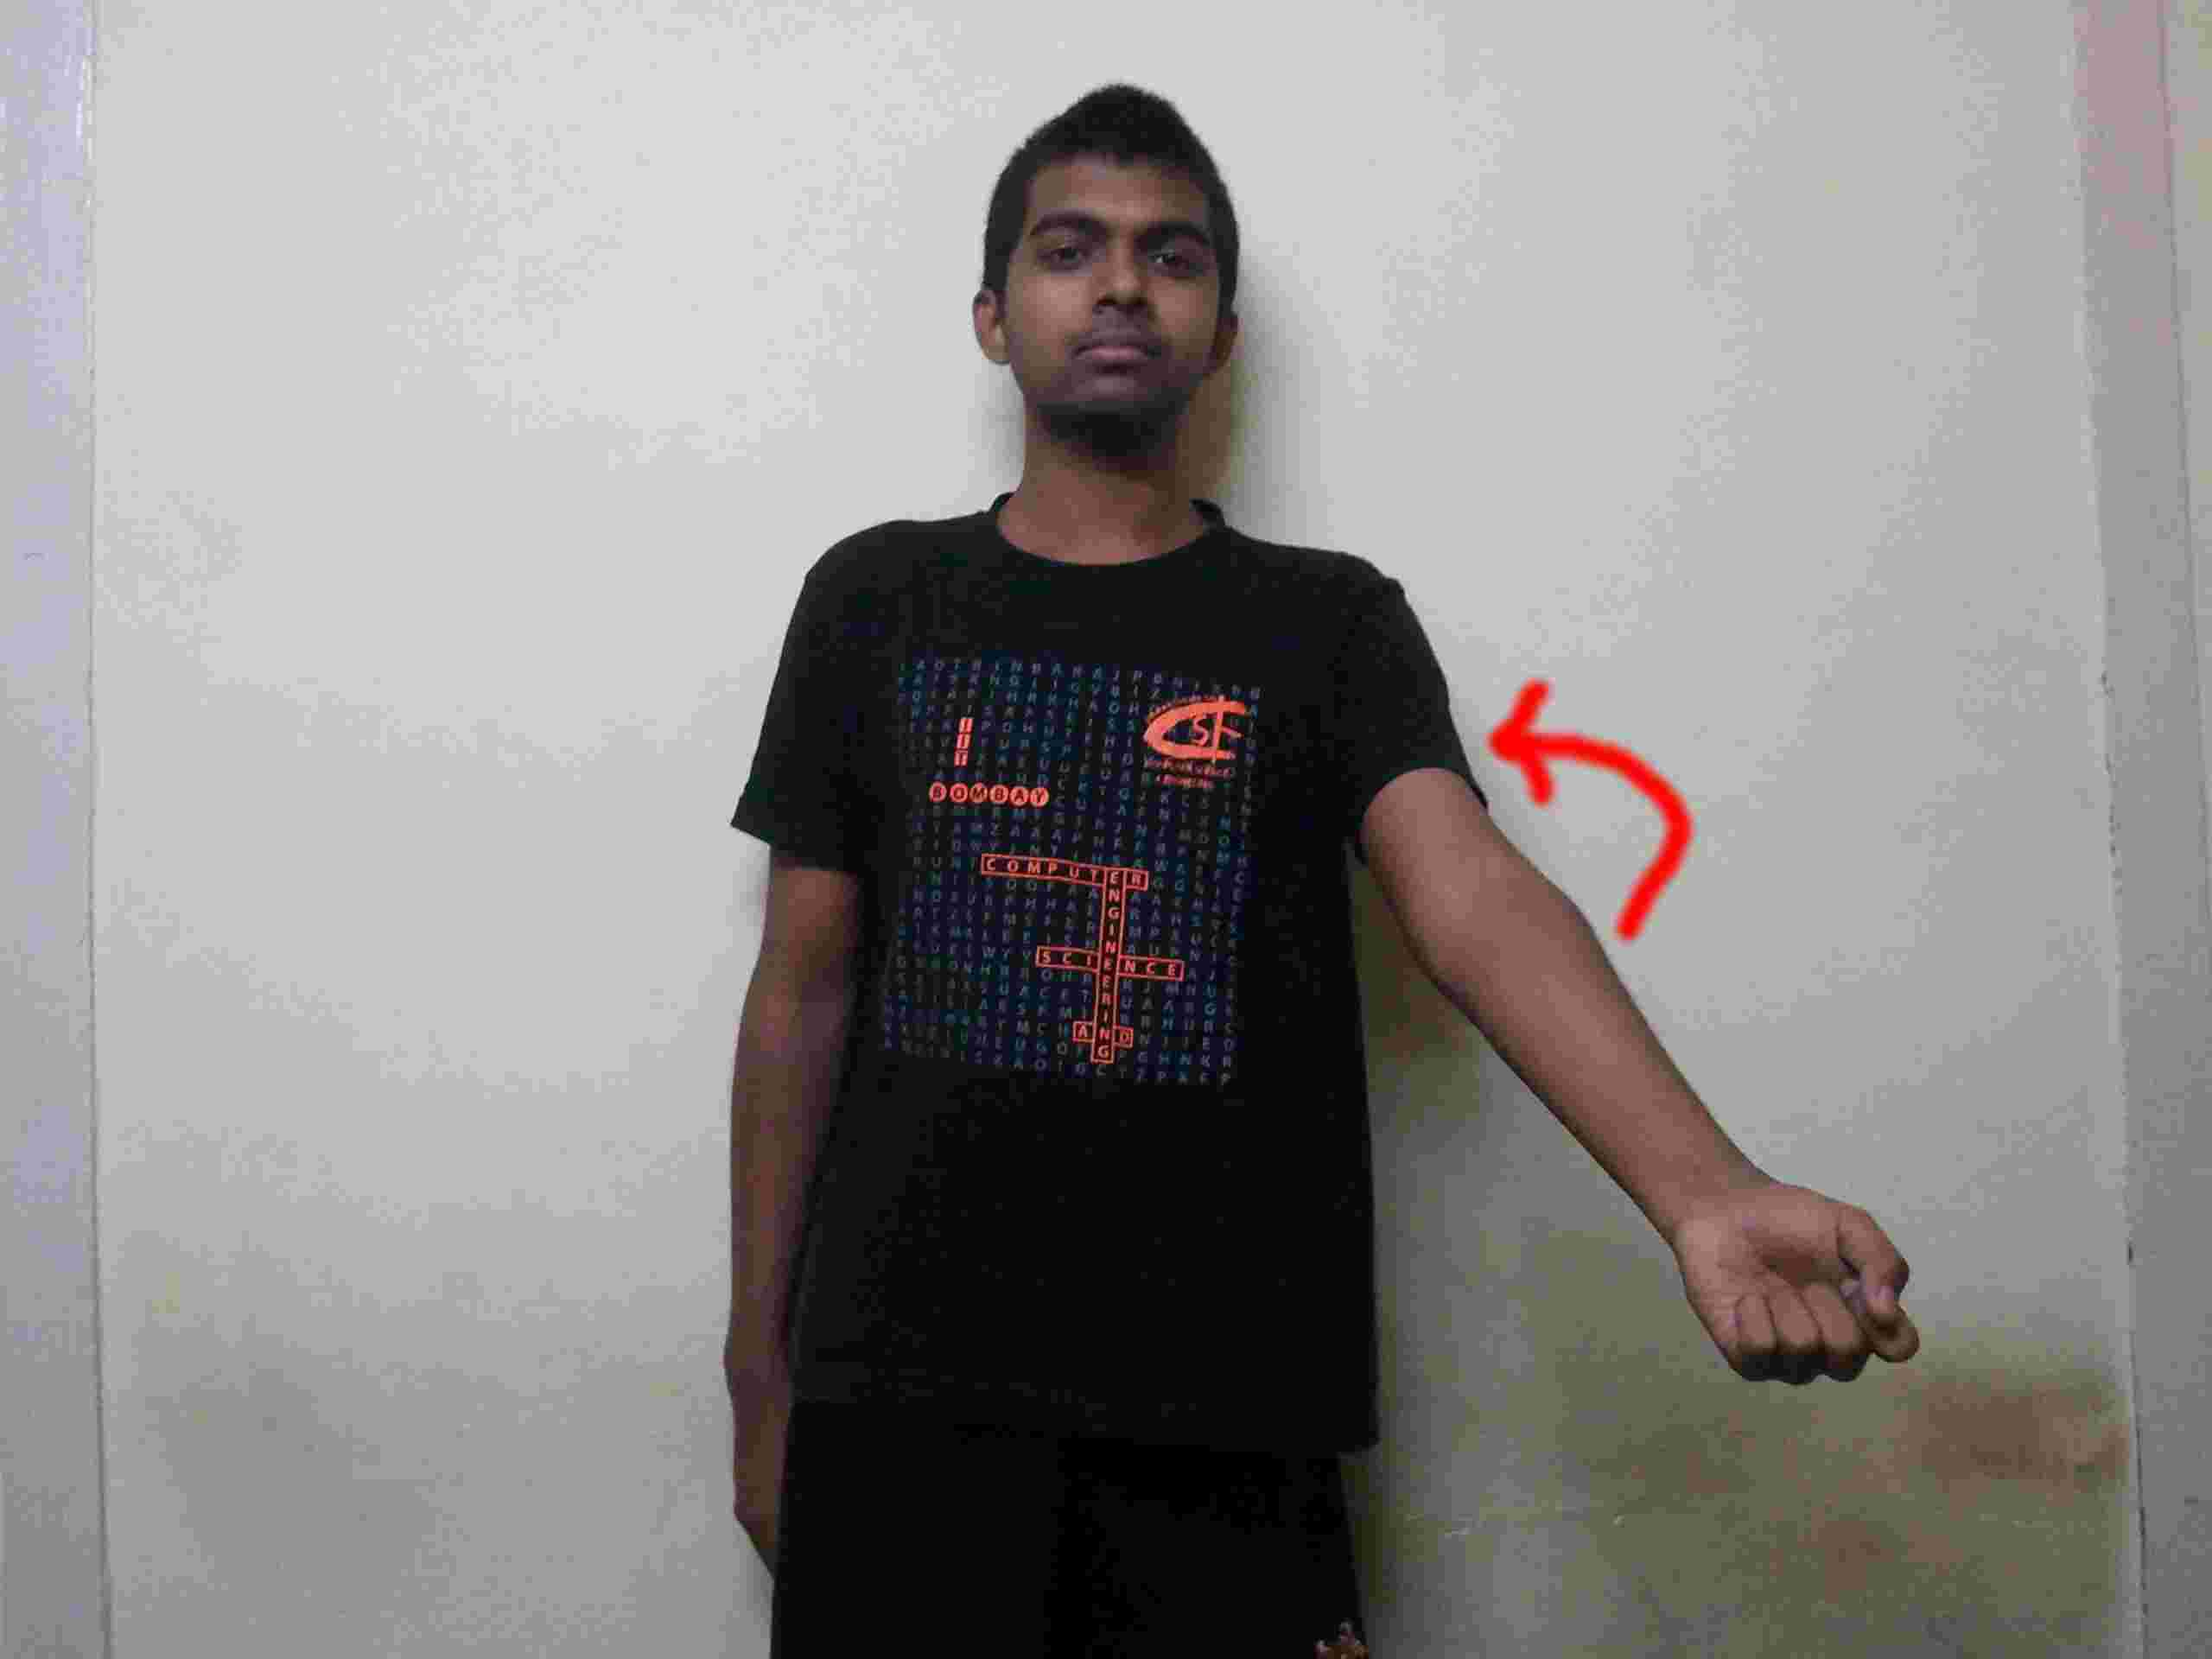
\includegraphics[scale=0.07]{gestures/61.jpg} &
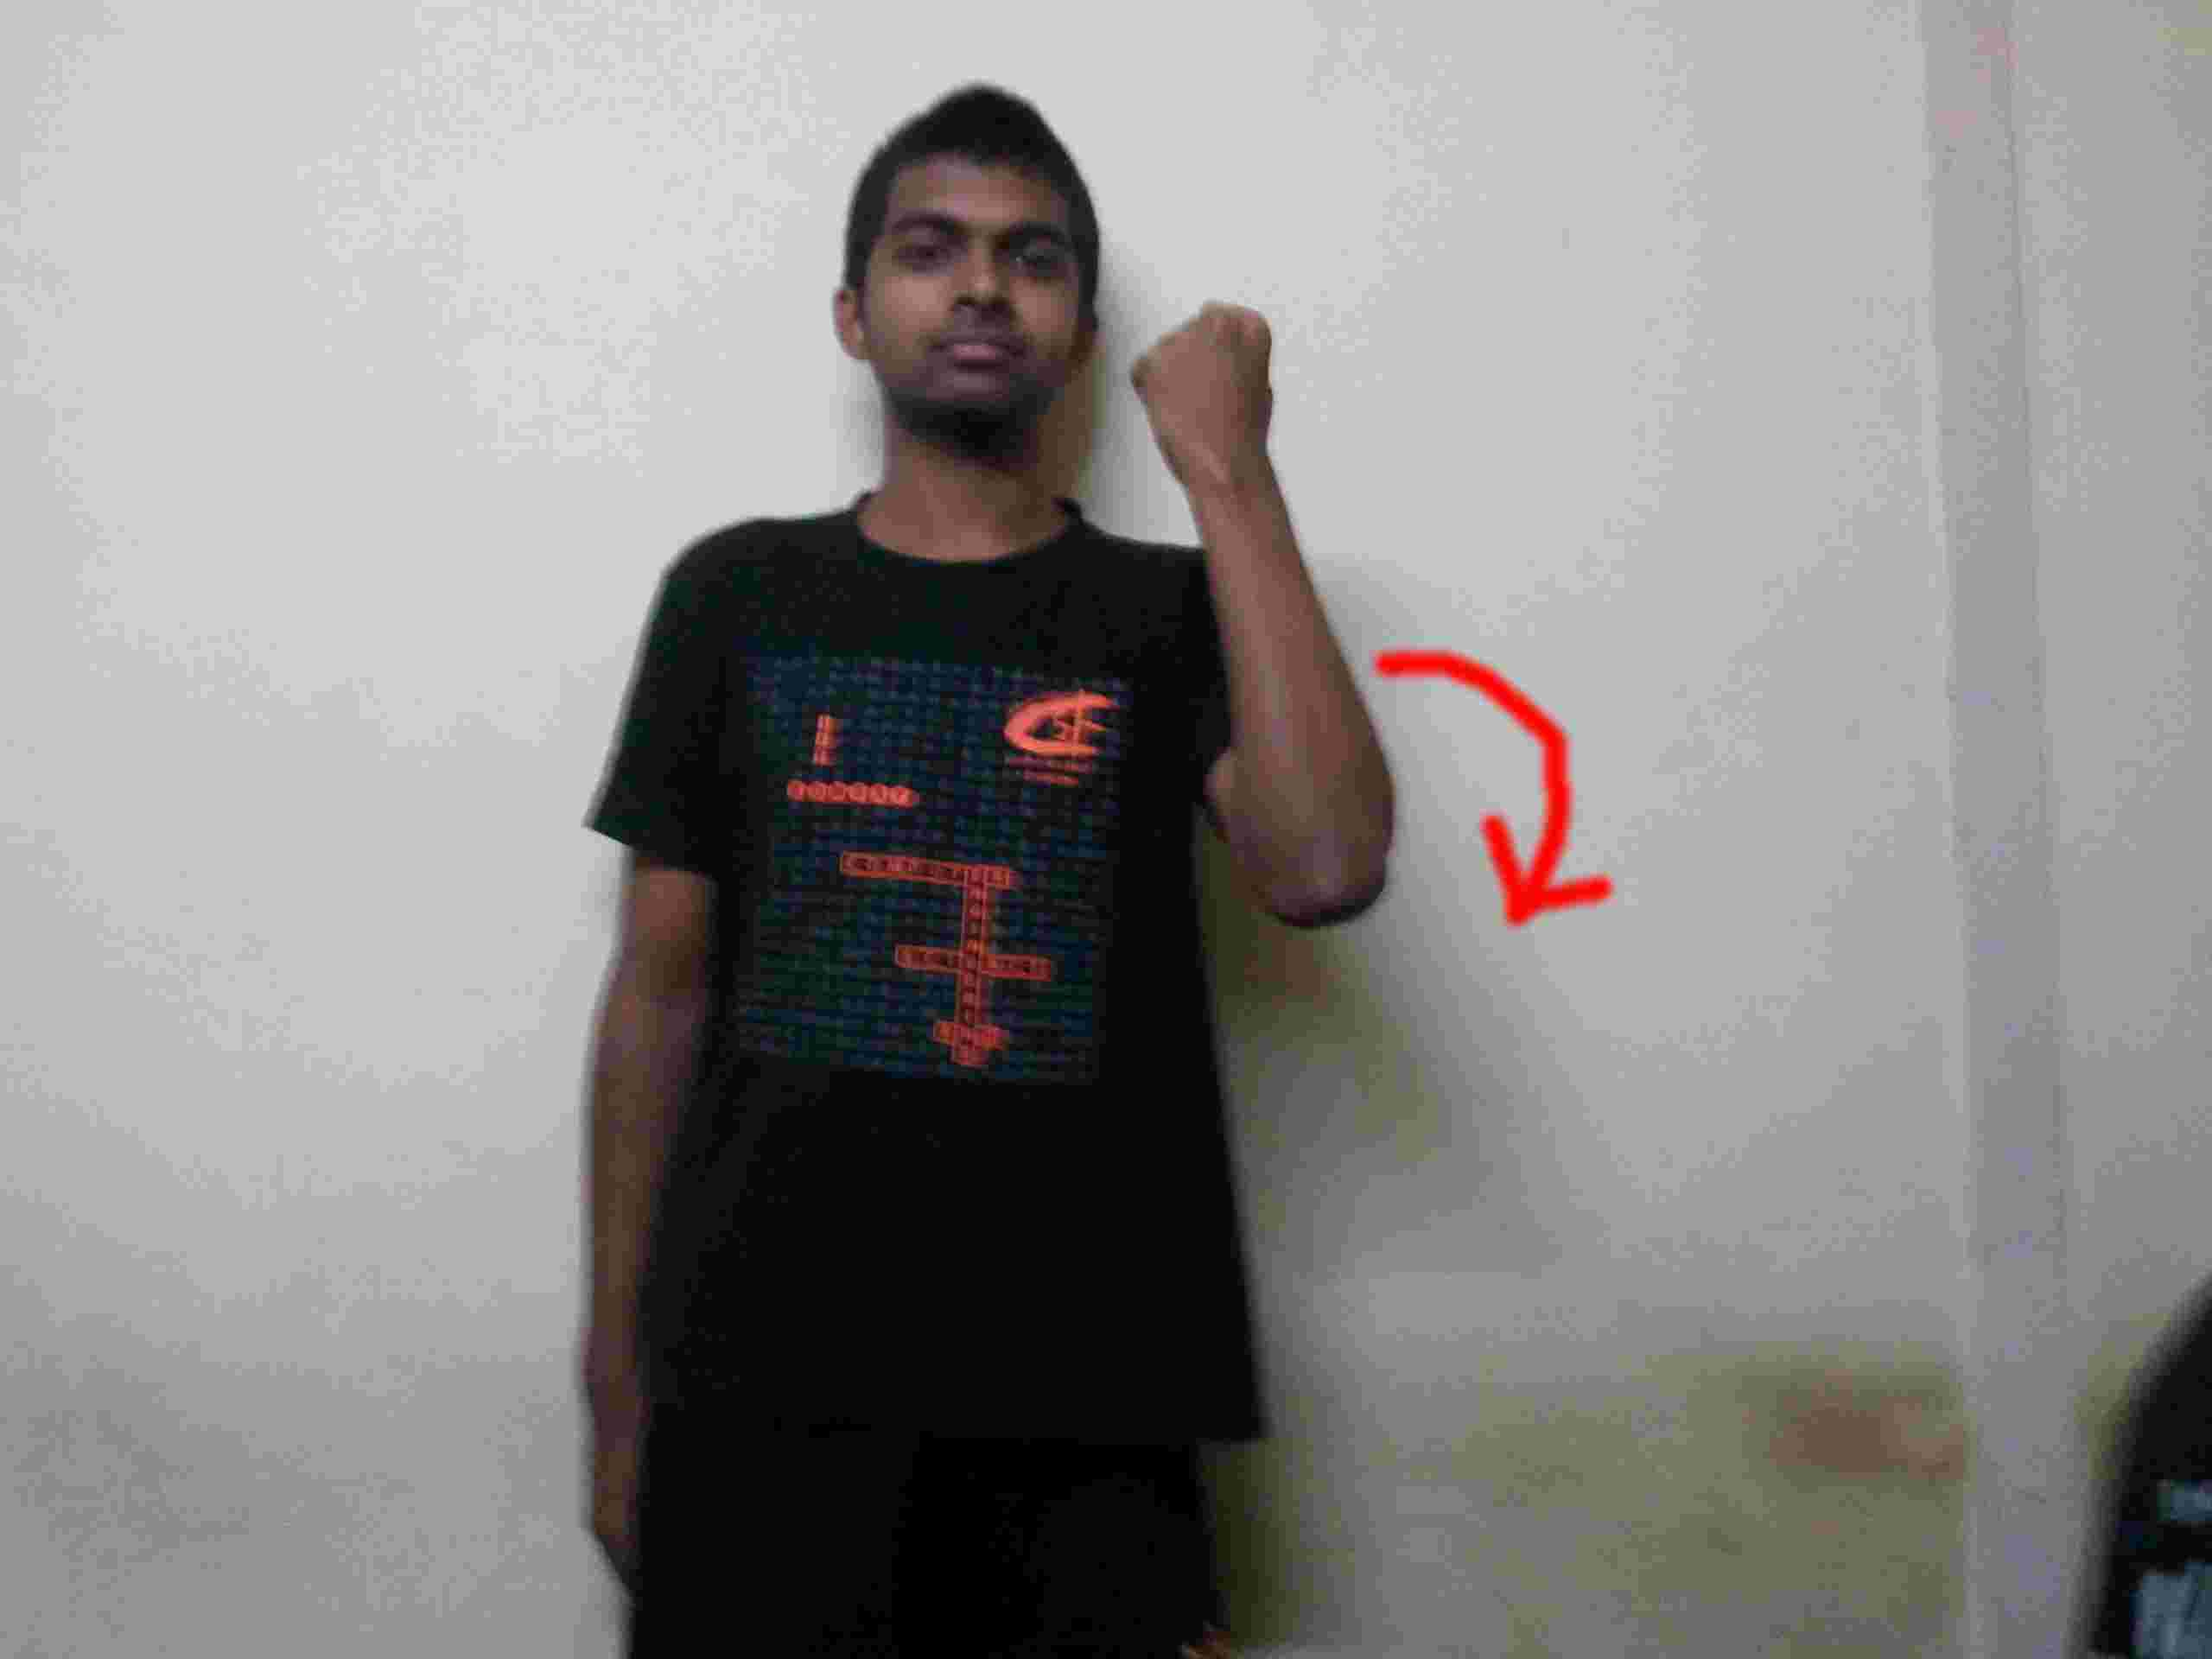
\includegraphics[scale=0.07]{gestures/62.jpg}
\end{array}
$
\end{figure}
%%%%%%%%%%%%%%%%%%%%%%%%%%%%%%%%%%%%%%%%%%%%%%%%%%%%%%%%%%%%%%%%%%%%%%%%%%%
\chapter{Details}
%%%%%%%%%%%%%%%%%%%%%%%%%%%%%%%%%%%%%%%%%%%%%%%%%%%%%%%%%%%%%%%%%%%%%%%%

\section{Functionality}
\indent Controlling a robotic arm with a traditional controller can be very difficult. It is very non-intuitive and increases the complexity of using the arm thus limiting its applications. With kinect the usability of the system is greatly enhanced because the natural movements of the human arm directly control the robotic arm which tries to imitate its movements. Thus controlling the arm becomes very intuitive and humans can readily use the robotic arm thus opening a plethora of applications.

\indent This system is designed to allow a user to control the robotic arm via remote wireless connectivity. A camera is mounted with the arm so that the user can see the environment of the arm and the arm itself as live video which will help the user control the arm better. This will enable the user to deploy the arm in remote or hostile places thus further multiplying the scope of applications. The wireless network is configured to provide point to point connectivity between the coordinator and the arm ensuring no external interference on the communication channel. 

\indent Kinect will facilitate recognition of the movement of the user arm to be detected as skeletal data which in turn are converted to signals used to control the arm.

%%%%%%%%%%%%%%%%%%%%%%%%%%%%%%%%%%%%%%%%%%%%%%%%%%%%%%%%%%%%%%%

\section{Supportability}

\subsection{Basis for future work}
\indent Because of its very general nature, this project can serve as the fundamental component of future projects exploring exciting applications opened up by this technology. Also we will try to abstract the most important parts of the system such that they are not specific to the robotic arm we are using or other specific details. So future projects can directly use this abstract high-level parts of our code without any modifications.

\subsection{Distinguished Modules of the Project}
\begin{itemize}
\item Kinect programming using Microsoft API for natural user interface for arm movement recognition
\item Controlling the robotic arm using ZigBee communication
\item Transmitting video data from remote camera to the coordinating computer
\end{itemize}

\subsection{Documentation}
 Documentation in terms of embedded comments and other explicit write-ups will
help others in future. We will try to provide high-level wrapping functions for all the important modules of our project and properly document them.

\section{Design Constraints}
The restrictions being implemented in the code are primarily due to those imposed of the system by the hardware being used. They are as follows:
\begin{itemize}
\item The human arm has an amazing degree of freedom and the robotic arm cannot exactly imitate. Thus we have to define appropriate actions for the arm for movements which directly do not correspond to human arm movements
\item It will be very difficult to represent finger movements even if the robotic arm supports it. But in our project we ignore this detail except for the actions corresponding to gripping and ungripping
\item The ZigBee Wireless Communication Module uses a Serial COM Ports. So, all the communication between the coordinator and the Robot will be via a serial port only
\item The ER2 robotic arm has a payload limit of 50gms. This makes the arm mechanically too week for any realistic work.
\item The ER2 robotic arm have a inbuilt Zigbee interface, so a Zigbee module needs to be attached to the arm for wireless control.
\item Microsoft Kinect SDK and DirectX SDK require Microsoft Visual Studios to be used to allow proper access of their libraries. So, the use of such SDKs will require Visual Studios explicitly

\end{itemize}

%%%%%%%%%%%%%%%%%%%%%%%%%%%%%%%%%%%%%%%%%%%%%%%%%%%%%%%%%%%%%%%%%%%%%

\section{Interfaces}

\subsection{User Interfaces}
This is the part of the system that will be used to interact with the user i.e. recognizing their arm movements as well as displaying information for them to be used for controlling the robotic arm. They are as follows:
\begin{itemize}
\item Kinect interface view of the user's arm  which includes the skeletal view, the camera view and the IR greyscale distance measurement view of the user's arm.
\item A display showing the camera view of the robotic arm and the environment.
\item The Robotic Arm GUI 
\end{itemize}

\subsection{Hardware Interfaces}
This section states the essential physical equipment required to interact with the application designed. They are as follows:
\begin{itemize}
\item Kinect Sensor Module to detect the movements of the user arm
\item Computer System with the following essentials are Kinect Sensor Module to run:
\begin{itemize}
\item  Intel Core2Duo 2.66GHz
\item  Dedicated VGA card with DirectX Support
\end{itemize}
\item A camera to be mounted with the robotic arm with the data bus connectivity to the ZigBee communication module.
\end{itemize}

\subsection{Software Interfaces}
This section states the requirements to develop the application which will use the data feed from the various interfaces and use them to control the arm or display information for the user. They are as follows:
\begin{itemize}
\item Kinect SDK which in turn requires the following:
\begin{itemize}
\item  Windows 7
\item  DirectX SDK
\end{itemize}
\item Visual Studios
\item Atmel AVR Studios
\item The Robotic Arm GUI
\end{itemize}

\subsection{Communications Interfaces}
This section states the requirements to create a communication between the robotic arm and the coordinator. They are as follows:
\begin{itemize}
\item 2 ZigBee Wireless Modules
\item X-CTU ZigBee Configuration
\end{itemize}

%%%%%%%%%%%%%%%%%%%%%%%%%%%%%%%%%%%%%%%%%%%%%%%%%%%%%%%%%%%%%%%%%%%%%%
\chapter{Quality Control}
%%%%%%%%%%%%%%%%%%%%%%%%%%%%%%%%%%%%%%%%%%%%%%%%%%%%%%%%%%%%%%%%%%%%%%
\subsection*{Accuracy of Skeletal Data}
The accuracy with which the arm can be controlled depends on the accuracy of the skeletal data obtained from Kinect. Better results can be obtained by considering the average over multiple frames.

\subsection*{Complexity of the Robotic Arm}
The accuracy with which movements of the human arm can be reproduced on the robotic arm is limited by the complexity of the robotic arm. For example, the robotic arm may not have an arrangement for rotation of the wrist.

\subsection*{Complexity of the Algorithm}
The skeletal structure of the human arm, and that of the robotic arm may be very different, and the accuracy of the reproduction of movements depends on the algorithm used to map movements about joints in the human arm to those in the robotic arm.
\subsection*{Calibration of Kinect for Gestures}
The kinect uses an IR sensor and accuracy of the depth data is limited by the calibration of the sensor.
%%%%%%%%%%%%%%%%%%%%%%%%%%%%%%%%%%%%%%%%%%%%%%%%%%%%%%%%%%%%%%%%%%%%%%
\chapter{Risk Management}
%%%%%%%%%%%%%%%%%%%%%%%%%%%%%%%%%%%%%%%%%%%%%%%%%%%%%%%%%%%%%%%%%%%%%%
\subsection*{Protection Against Large/Fast Movements}
Large or very fast movements of the human arm, if reproduced directly, can cause damage to the robotic arm. Care must be taken to limit the speed of movement and the range of angles covered by the robotic arm.

\subsection*{Protection Against Wear and Tear}
The motors used at the joints may may be suffer damage if used continuously for extended periods of time. To prevent this, the motors must be automatically turned off when idle.

\subsection*{Protection Against Heavy Payload}
The ER2 robotic arm has a payload limit of 50gms. Heavier payloads may cause damage to the motors. Care must be taken not to exceed this limit.

\subsection*{Problems with Calibration}
Miscalibration of the depth sensor of Kinect can lead to incorrect and unexpected results. To avoid this, the calibration of the sensor must be checked regularly.

\subsection*{Problems with Gesture Recognition}
A single pattern made by the user will never be an exact match to itself
if tried repeatedly. So, the recognition program will have to be sufficiently lenient so as to allow some liberties to the user but not to misinterpret a general movement for a gesture. So, in order to confirm a gesture, a trial run will be needed prior to using the bot to confirm the movement pattern is recognizable as a gesture during the trial runs.

%%%%%%%%%%%%%%%%%%%%%%%%%%%%%%%%%%%%%%%%%%%%%%%%%%%%%%%%%%%%%%%%%%%%%%%
\end{document}
